\chapter{ImProver 2 Experiments}\label{chap:improver2-exp}

\setlength{\parindent}{1em}


\subsection{Setup}
\label{sec:exp_setup}

We evaluate ImProver 2\ on all three metrics using public research-level
mathematics repositories, benchmarking against open-source and closed-source
baselines at varying parameter counts.

\subsubsection{Dataset and split}


We utilize Lean proofs from several open-source projects formalizing research-level mathematics across multiple domains \cite{Mathlib, HEPLean, PFR, Carleson, ConNF, FLT, Foundation, Seymour}. We hold out all theorems in miniCTX-v2 as the test set. To prevent
data leakage, we additionally exclude from training every theorem
that appears in the same source file as a miniCTX-v2 theorem.
Training and validation sets are drawn from all remaining files
in an $80\%/20\%$ split, although we pre-filter the Mathlib portion of the dataset to a uniformly sampled subset of 37 files, due to its significantly larger scale.

We believe miniCTX-v2 represents a reasonable approximation of the problems that would be encountered during deployment for optimizing human-written research-level math. Although we hypothesize that ImProver 2 \ could perform similar optimization in other domains, such as long machine-generated proofs, we omit testing on these domains as they fall outside the scope of the aforementioned application. 

\subsubsection{Evaluation protocol}

For all main results, we evaluate with best@16 sampling (Definition~\ref{def:best_of_n}) and report the mean improvement score $\overline{S}_\mu(\mathcal{D}_{\mathrm{test}})$ (Definition~\ref{def:mean_improvement}) for $\mu \in \{\mu_{\mathrm{len}}, \mu_{\mathrm{dep}}, \mu_{\mathrm{mod}}\}$. We also report compilation accuracy $\mathcal{A}(\mathcal{D}_{\mathrm{test}})$ (Definition~\ref{def:comp_acc}) and improved accuracy $\mathcal{A}^+_\mu(\mathcal{D}_{\mathrm{test}})$ (Definition~\ref{def:imp_acc}). We operate with a base model of $G_0 = \texttt{DeepSeek-R1-Distill-Qwen-7B}$~\cite{DeepseekR1}. Hyperparameters and configuration are described in \cite{ImProver2}.


\subsubsection{Systems compared}


\begin{table}
\centering
\caption{Inference cost comparison, based on public API pricing at 
time of submission, and given as the Input/Output cost per 1M tokens.}
\small
\begin{tabular}{lcccc}
\toprule
\textbf{Model} & \textbf{Type} & \textbf{Cost}\\
\midrule
DeepSeek-R1-7B & Open-weight & Locally Hosted \\
DeepSeek-R1-14B & Open-weight & Locally Hosted \\
DeepSeek-R1-671B & Open-weight & \$0.70/ \$2.50 \\
GPT-4o & API & \$2.50 / \$10 \\
GPT-5-nano & API & \$0.05 / \$0.40 \\
GPT-5-mini & API & \$0.25 / \$2\\
GPT-oss-120B & Open-weight & Locally Hosted \\
GPT-5-chat & API & \$1.25 /\$10   \\
GPT-5 (High) & API & \$1.25 / \$10  \\
\bottomrule
\end{tabular}
\label{tab:cost}
\end{table}

Our main evaluation compares ImProver 2\ against three classes of baselines on MiniCTX-v2 under best@16 sampling: (i) the \texttt{DeepSeek-R1} family at multiple scales, to study parameter scaling within a fixed model family; (ii) frontier GPT-based and open-weight systems, including \texttt{GPT-5-high} (a full-size high-reasoning variant), \texttt{GPT-5-chat}, \texttt{GPT-5-mini}, \texttt{GPT-5-nano}, and \texttt{GPT-oss-120B}; and (iii) the prior \texttt{ImProver} system and its base model \texttt{GPT-4o}. Current inference costs for each system is displayed in Table~\ref{tab:cost}.


We also evaluate all generators with and without the neurosymbolic scaffold $\Psi$ to isolate the effect of augmentation from the effect of training.
For each metric, we train IRPO until validation improvement regresses and report the best checkpoint for that objective.

% We formulate our main results to compare several iterations of ImProver 2's IRPO pipeline on MiniCTX-v2, evaluated on the best@16 improvement score across all three metrics. In particular, we compare ImProver 2 to (i) its \texttt{DeepSeek-R1} model family across various parameter sizes; (ii) frontier GPT-based models such as \texttt{GPT-5-chat} (a nonreasoning variant of \texttt{GPT-5}, chosen due to resource constraints), \texttt{GPT-5-mini}, \texttt{GPT-5-nano}, and \texttt{GPT-oss-120B}; and (iii) prior work on proof optimization, namely, \texttt{ImProver} and its base model \texttt{GPT-4o}. We additionally augment all the aforementioned models with our neurosymbolic scaffold $\Psi$ and similarly compare its best@16 mean improvement score to the unscaffolded version.

% For each metric, we ran IRPO iterations until mean improvement
% on the validation set regressed, then selected the
% best-performing checkpoint (iteration 3 for length, 2 for
% dependency, and 3 for modularity; see Table~\ref{tab:iter}).

% We additionally perform a robust ablation study of the effects of the neurosymbolic augmentation on various metrics, as well as a full grid search evaluation and optimization of all hyperparameters in our training pipeline.

% And lastly, we showcase a collection of selected qualitative results across datasets and metrics to study the high-level behaviors and emergent optimization patterns of the final ImProver 2~ system.

\subsection{Main Results}
\label{sec:main_results}



\begin{table}
\centering
\caption{\textbf{Frontier Evaluations.} Comparison with frontier models and prior proof optimization systems. Mean improvement at best@16 on MiniCTX-v2}
\small
\begin{tabular}{l|cccc}
\hline
\textbf{Model}  & \textbf{Length} & \textbf{Mod.} & \textbf{Dep.} \\
\hline
GPT-4o & 0.336 & 0.034 & 0.050  \\ 
GPT-oss-120B & 0.321 & 0.075 & 0.181  \\
GPT-5-nano  & 0.087 & 0.065 & 0.106 \\
GPT-5-mini   & 0.330 & 0.109 & 0.203  \\
GPT-5-chat  & 0.346 & 0.118 & 0.046  \\
GPT-5-high  & \textbf{0.660} & 0.120 & \textbf{0.208}  \\
\hdashline
ImProver & 0.355 & 0.088 & 0.047  \\ 
ImProver 2  & 0.330 & \textbf{0.143} & 0.206  \\

\hline
\end{tabular}
\label{tab:frontier}
\end{table}



\begin{table}
\centering
\caption{\textbf{Intra-Family Evaluations.} Intra-family comparison across DeepSeek-R1 model scales. Mean improvement at best@16 on MiniCTX-v2 for all three metrics.}
\small
\begin{tabular}{l|cccc}
\hline
\textbf{Model}  & \textbf{Length} & \textbf{Mod.} & \textbf{Dep.} \\
\hline
DeepSeek-R1 7B     & 0.118 & 0.003 & 0.050  \\ 
DeepSeek-R1 14B      & 0.140 & 0.037 & 0.093  \\
DeepSeek-R1 671B & 0.308 & 0.055 & 0.153  \\
\hdashline
ImProver 2  & \textbf{0.330} & \textbf{0.143} & \textbf{0.206}  \\
\hline
\end{tabular}
\label{tab:intrafamily}
\end{table}



Tables~\ref{tab:frontier} and \ref{tab:intrafamily} show that ImProver 2\ substantially improves over its 7B base generator on all three objectives, leads all evaluated unscaffolded systems on modularity, and is competitive with frontier models on dependency and length.


After IRPO training, ImProver 2\ achieves mean best@16 improvements of $0.330$ on 
length, $0.143$ on modularity, and $0.206$ on dependency, compared to $0.118$, 
$0.003$, and $0.050$ for the untrained \texttt{DeepSeek-R1 7B} baseline.
These correspond to roughly $2.8\times$ on length, $4.1\times$ on dependency, and 
a large absolute gain on modularity ($0.003 \to 0.143$). We note that the 
dependency multiplier reflects both the effectiveness of the pipeline and the 
low absolute baseline of the untrained model. Together, 
these gains indicate that iterative self-improvement combined with neurosymbolic 
conditioning yields substantial improvements even from a 7B base model.

These gains are not confined to a single objective.
While length improves steadily with model scale, ImProver 2\ also delivers strong gains on the more structural objectives of dependency and modularity, which require more than local proof compression.
In particular, its dependency score of $0.206$ exceeds both the 14B and 671B DeepSeek baselines, suggesting that for structural proof refactoring, task-specific training can matter at least as much as raw parameter count.

Comparison with frontier systems further sharpens this picture. On modularity, ImProver 2\ leads all unscaffolded systems evaluated at $0.143$, 
ahead of the next-best frontier models (\texttt{GPT-5} high reasoning at $0.120$, \texttt{GPT-5-chat} at $0.118$), suggesting that iterative task-specific 
training can catch up to raw model scaling for learning to decompose proofs into 
reusable subproof structure.
Similarly, on dependency, ImProver 2\ is competitive with the strongest frontier systems: 
it achieves $0.206$, essentially tied with \texttt{GPT-5-high} ($0.208$) and 
ahead of \texttt{GPT-5-mini} ($0.203$).
On length, ImProver 2\ ($0.330$) is competitive with mid-tier frontier models, 
matching \texttt{GPT-5-mini} ($0.330$) and exceeding \texttt{GPT-oss-120B} 
($0.321$), while trailing only \texttt{GPT-5-high} ($0.660$) — a full-size 
high-reasoning variant operating at substantially greater inference cost — by 
a significant margin. The prior \texttt{ImProver} system ($0.355$) also leads 
on length, consistent with its use of an agentic prompting strategy on a substantially larger \texttt{GPT-4o} base model, specifically optimized for proof shortening.

Overall, the results suggest that task-specific iterative training is particularly 
effective for structural refactoring: ImProver 2\ leads all systems on modularity 
and is competitive with the strongest frontier models on dependency, while 
remaining within range of mid-tier frontier models on length --- all from just a completely bootstrapped training pipeline on a 7B base model.



\begin{table}
\centering
\caption{\textbf{Per-iteration improvements.} Progression of mean improvement at best@16 on MiniCTX-v2 across IRPO training iterations across all three metrics.}
\small
\begin{tabular}{lccc}
\hline
\textbf{Iteration} & \textbf{Length}  & \textbf{Mod.}  & \textbf{Dep.}  \\
\hline
Base     & 0.118 & 0.003 & 0.050  \\ 
\textit{+ Scaffold} & 0.236 & 0.007 & 0.056  \\
\hdashline
1   & 0.265 & 0.062 & 0.137  \\
2   & 0.318  & 0.134 & \textbf{0.206}  \\
3   & \textbf{0.330}  & \textbf{0.143} & 0.165  \\
4   & 0.299 & 0.096 & N/A \\
\hline
\end{tabular}
\label{tab:iter}
\end{table}



\subsection{Improvement vs Accuracy}
\label{sec:acc}

Mean improvement alone does not distinguish between broad, reliable gains and a smaller set of high-reward successes.
We therefore also report compilation accuracy $\mathcal{A}$ and improved accuracy $\mathcal{A}_\mu^+$, where $\mathcal{A}_\mu^+$ measures the fraction of test problems for which the model produces a compiling proof that has a strictly positive metric improvement score.

Across both models and training iterations, optimization tends to raise $\mathcal{A}_\mu^+$ faster than $\mathcal{A}$.
This is especially visible in the iteration study (Table~\ref{tab:iter_acc}).
For dependency minimization, the base model begins with high compilation accuracy but low improved accuracy ($0.754$ and $0.037$ respectively), indicating that it often produces valid rewrites without meaningfully reducing dependency footprint.
After training, improved accuracy rises sharply, peaking at $0.106$ in iteration 2, while compilation accuracy drops to $0.464$.
This reflects a central tradeoff of proof refactoring: larger structural edits are more likely to yield real gains when they succeed, but they also create more opportunities for compilation failure.

The same pattern appears in cross-model comparisons.
For example, \texttt{GPT-5-nano} attains very high compilation accuracy on dependency ($0.894$) but only moderate improved accuracy ($0.065$), whereas ImProver 2\ attains lower compilation accuracy ($0.368$) but slightly higher improved accuracy ($0.069$).
This suggests that conservative models often preserve correctness by making safer edits, while specialized optimizers are more willing to attempt riskier transformations that improve the target metric when successful.
Accordingly, we view $\mathcal{A}$ and $\mathcal{A}_\mu^+$ as complementary: $\mathcal{A}$ measures stability, while $\mathcal{A}_\mu^+$ more directly captures whether the system is solving the optimization problem rather than merely preserving compilability.

\begin{table}
\centering
\caption{\textbf{Accuracy Evaluations.} Compilation accuracy and improved accuracy comparison amongst the best@16 mean improvement samples across all three metrics. Each entry is reported as $\mathcal{A}_\mu^+ / \mathcal{A}$, where $\mathcal{A}_\mu^+$ is improved accuracy and $\mathcal{A}$ is compilation accuracy.}
\small
\setlength{\tabcolsep}{5pt}
\begin{tabular}{l|ccc}
\hline
\textbf{Model} & \textbf{Length} & \textbf{Mod.} & \textbf{Dep.} \\
\hline
DS-R1 7B      & 0.062 / 0.617 & 0.003 / 0.570 & 0.037 / 0.754 \\
DS-R1 14B     & 0.075 / 0.660 & 0.034 / \textbf{0.775} & 0.065 / 0.567 \\
DS-R1 671B  & 0.162 / 0.536 & 0.048 / 0.536 & 0.109 / 0.480 \\
\hline
ImProver 2 & 0.131 / 0.657 & 0.065 / 0.579 & 0.069 / 0.368 \\
\hline
ImProver            & 0.171 / 0.560 & 0.068 / 0.597 & 0.031 / 0.249 \\
GPT-4o              & 0.158 / 0.595 & 0.031 / 0.464 & 0.028 / 0.227 \\
GPT-oss        & 0.171 / 0.692 & 0.068 / 0.477 & 0.097 / 0.676 \\
GPT-5-nano          & 0.044 / 0.461 & 0.053 / 0.757 & 0.065 / \textbf{0.894} \\
GPT-5-mini          & 0.159 / 0.623 & 0.085 / 0.525 & \textbf{0.111} / 0.834 \\
GPT-5-chat          & 0.165 / 0.586 & 0.084 / 0.455 & 0.025 / 0.185 \\
GPT-5-high          & \textbf{0.264} / \textbf{0.757} & \textbf{0.092} / 0.656 & 0.094 / 0.753 \\
\hline
\end{tabular}
\label{tab:acc}
\end{table}


\begin{table}
\centering
\caption{\textbf{Accuracy Progression.} Compilation accuracy and improved accuracy progression amongst the best@16 mean improvement samples across IRPO training iterations. Each entry is reported as $\mathcal{A}_\mu^+ / \mathcal{A}$, where $\mathcal{A}_\mu^+$ is improved accuracy and $\mathcal{A}$ is compilation accuracy.}
\small
\setlength{\tabcolsep}{5pt}
\begin{tabular}{l|ccc}
\hline
\textbf{Model} & \textbf{Length} & \textbf{Mod.} & \textbf{Dep.} \\
\hline
Base      & 0.062 / 0.617 & 0.003 / 0.570 & 0.037 / 0.754 \\
\hline
Iter. 1 & 0.125 / 0.720 & 0.044 / \textbf{0.679} & 0.093 / 0.417 \\
Iter. 2 & \textbf{0.131} / 0.679 &\textbf{ 0.121} / 0.614 & \textbf{0.106} / \textbf{0.464} \\
Iter. 3 & 0.121 / \textbf{0.682} & 0.118 / 0.579 & 0.069 / 0.368 \\
Iter. 4 & \textbf{0.131} / 0.657 & 0.065 / 0.579 & N/A \\

\hline
\end{tabular}
\label{tab:iter_acc}
\end{table}


\subsection{Performance and Parameter Scaling}
\label{sec:perf_param}

A central question is whether proof optimization performance is primarily driven by scale or by task-specific specialization, when all else is equal. Figure~\ref{fig:param_perf} shows that within the \texttt{DeepSeek-R1} model family, larger models generally achieve higher mean improvement under a fixed prompting and sampling protocol. This trend is clearest for length and dependency, indicating that generic reasoning capacity does help with proof refactoring.

At the same time, scale is not the full story. ImProver 2, trained from a 7B base model, outperforms the much larger 671B DeepSeek model on all three objectives. The gap is especially pronounced for modularity ($0.143$ vs.\ $0.055$) and dependency ($0.206$ vs.\ $0.153$), suggesting that for structural proof optimization, the relevant bottleneck is not only reasoning capacity but also whether the model has been adapted to the structure of the formal task.

This interpretation is reinforced by the accuracy metrics. Namely, within the same model family, larger general-purpose models often maintain stronger raw compilation rates, but ImProver 2\ is more likely to produce compiling proofs that are also improved under the target metric.

We therefore interpret the scaling results as evidence that proof optimization is only partly a scale problem; it is also a specialization problem, and one for which iterative preference optimization is particularly effective.



\begin{figure*}
\centering
\begin{minipage}{0.49\linewidth}
    \centering
    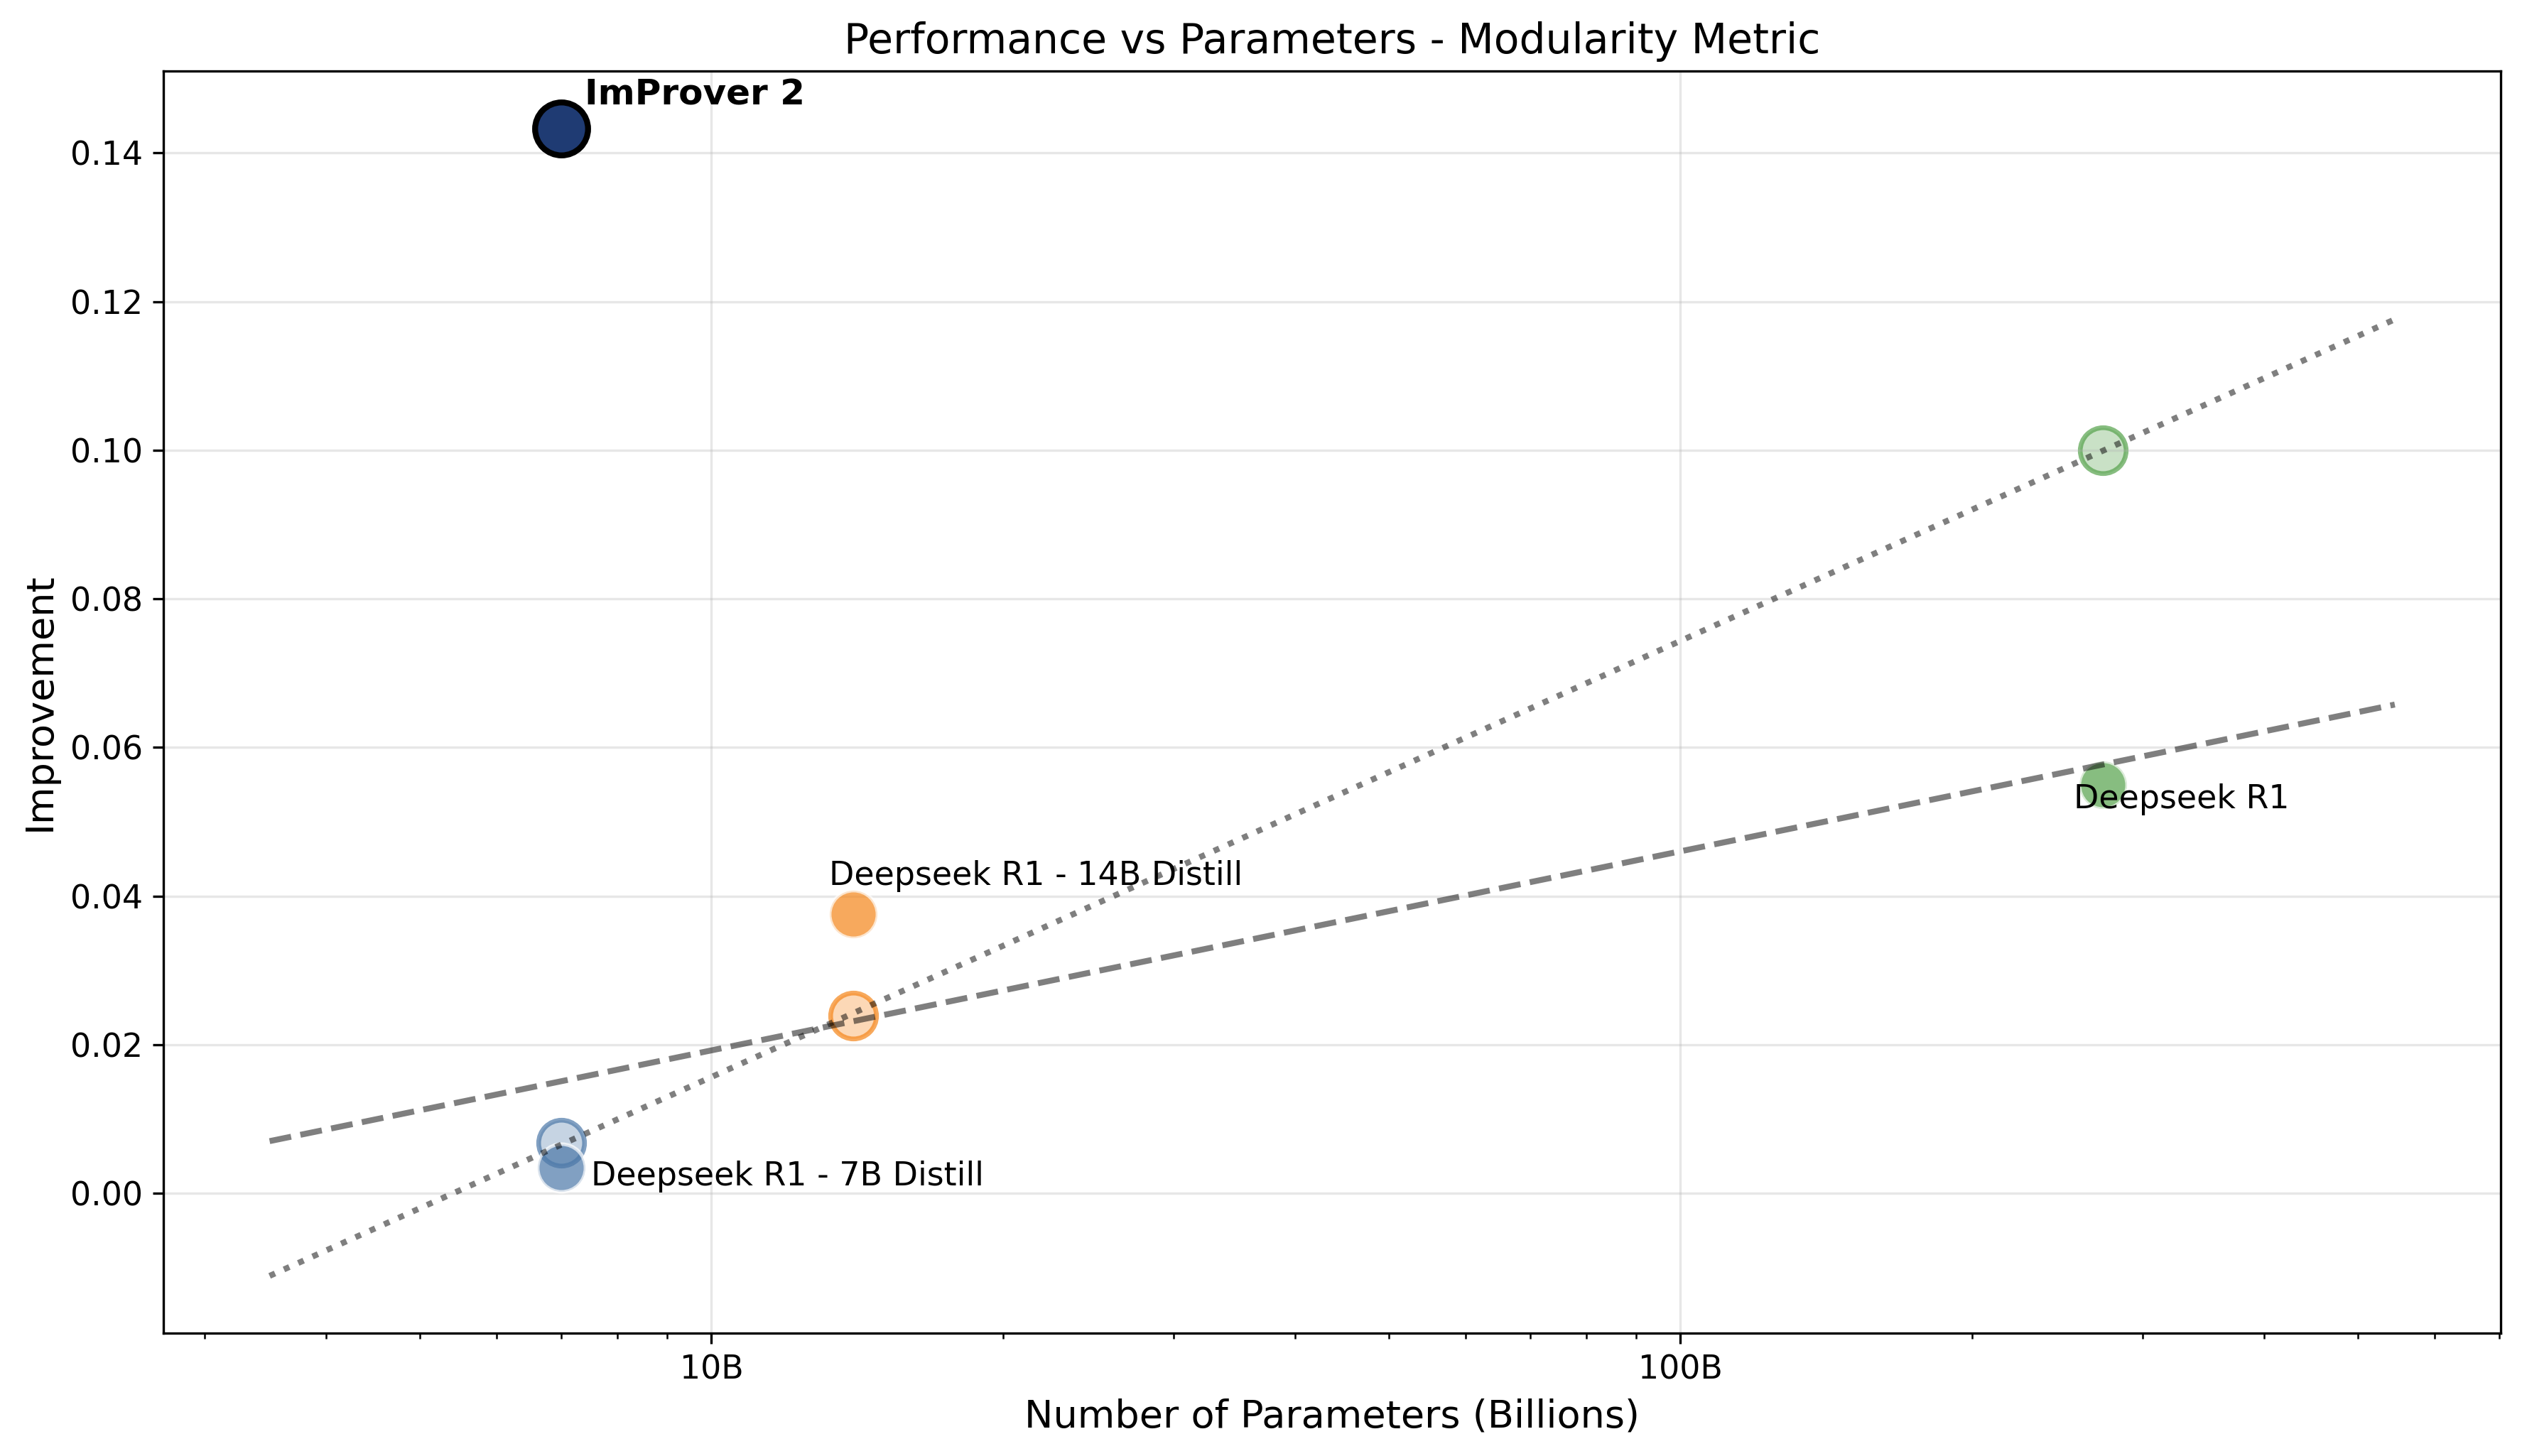
\includegraphics[width=1\linewidth]{figures/Modularity/declarativity2_param_perf.png}
    
\end{minipage}
% \hfill
\begin{minipage}{0.49\linewidth}
    \centering
    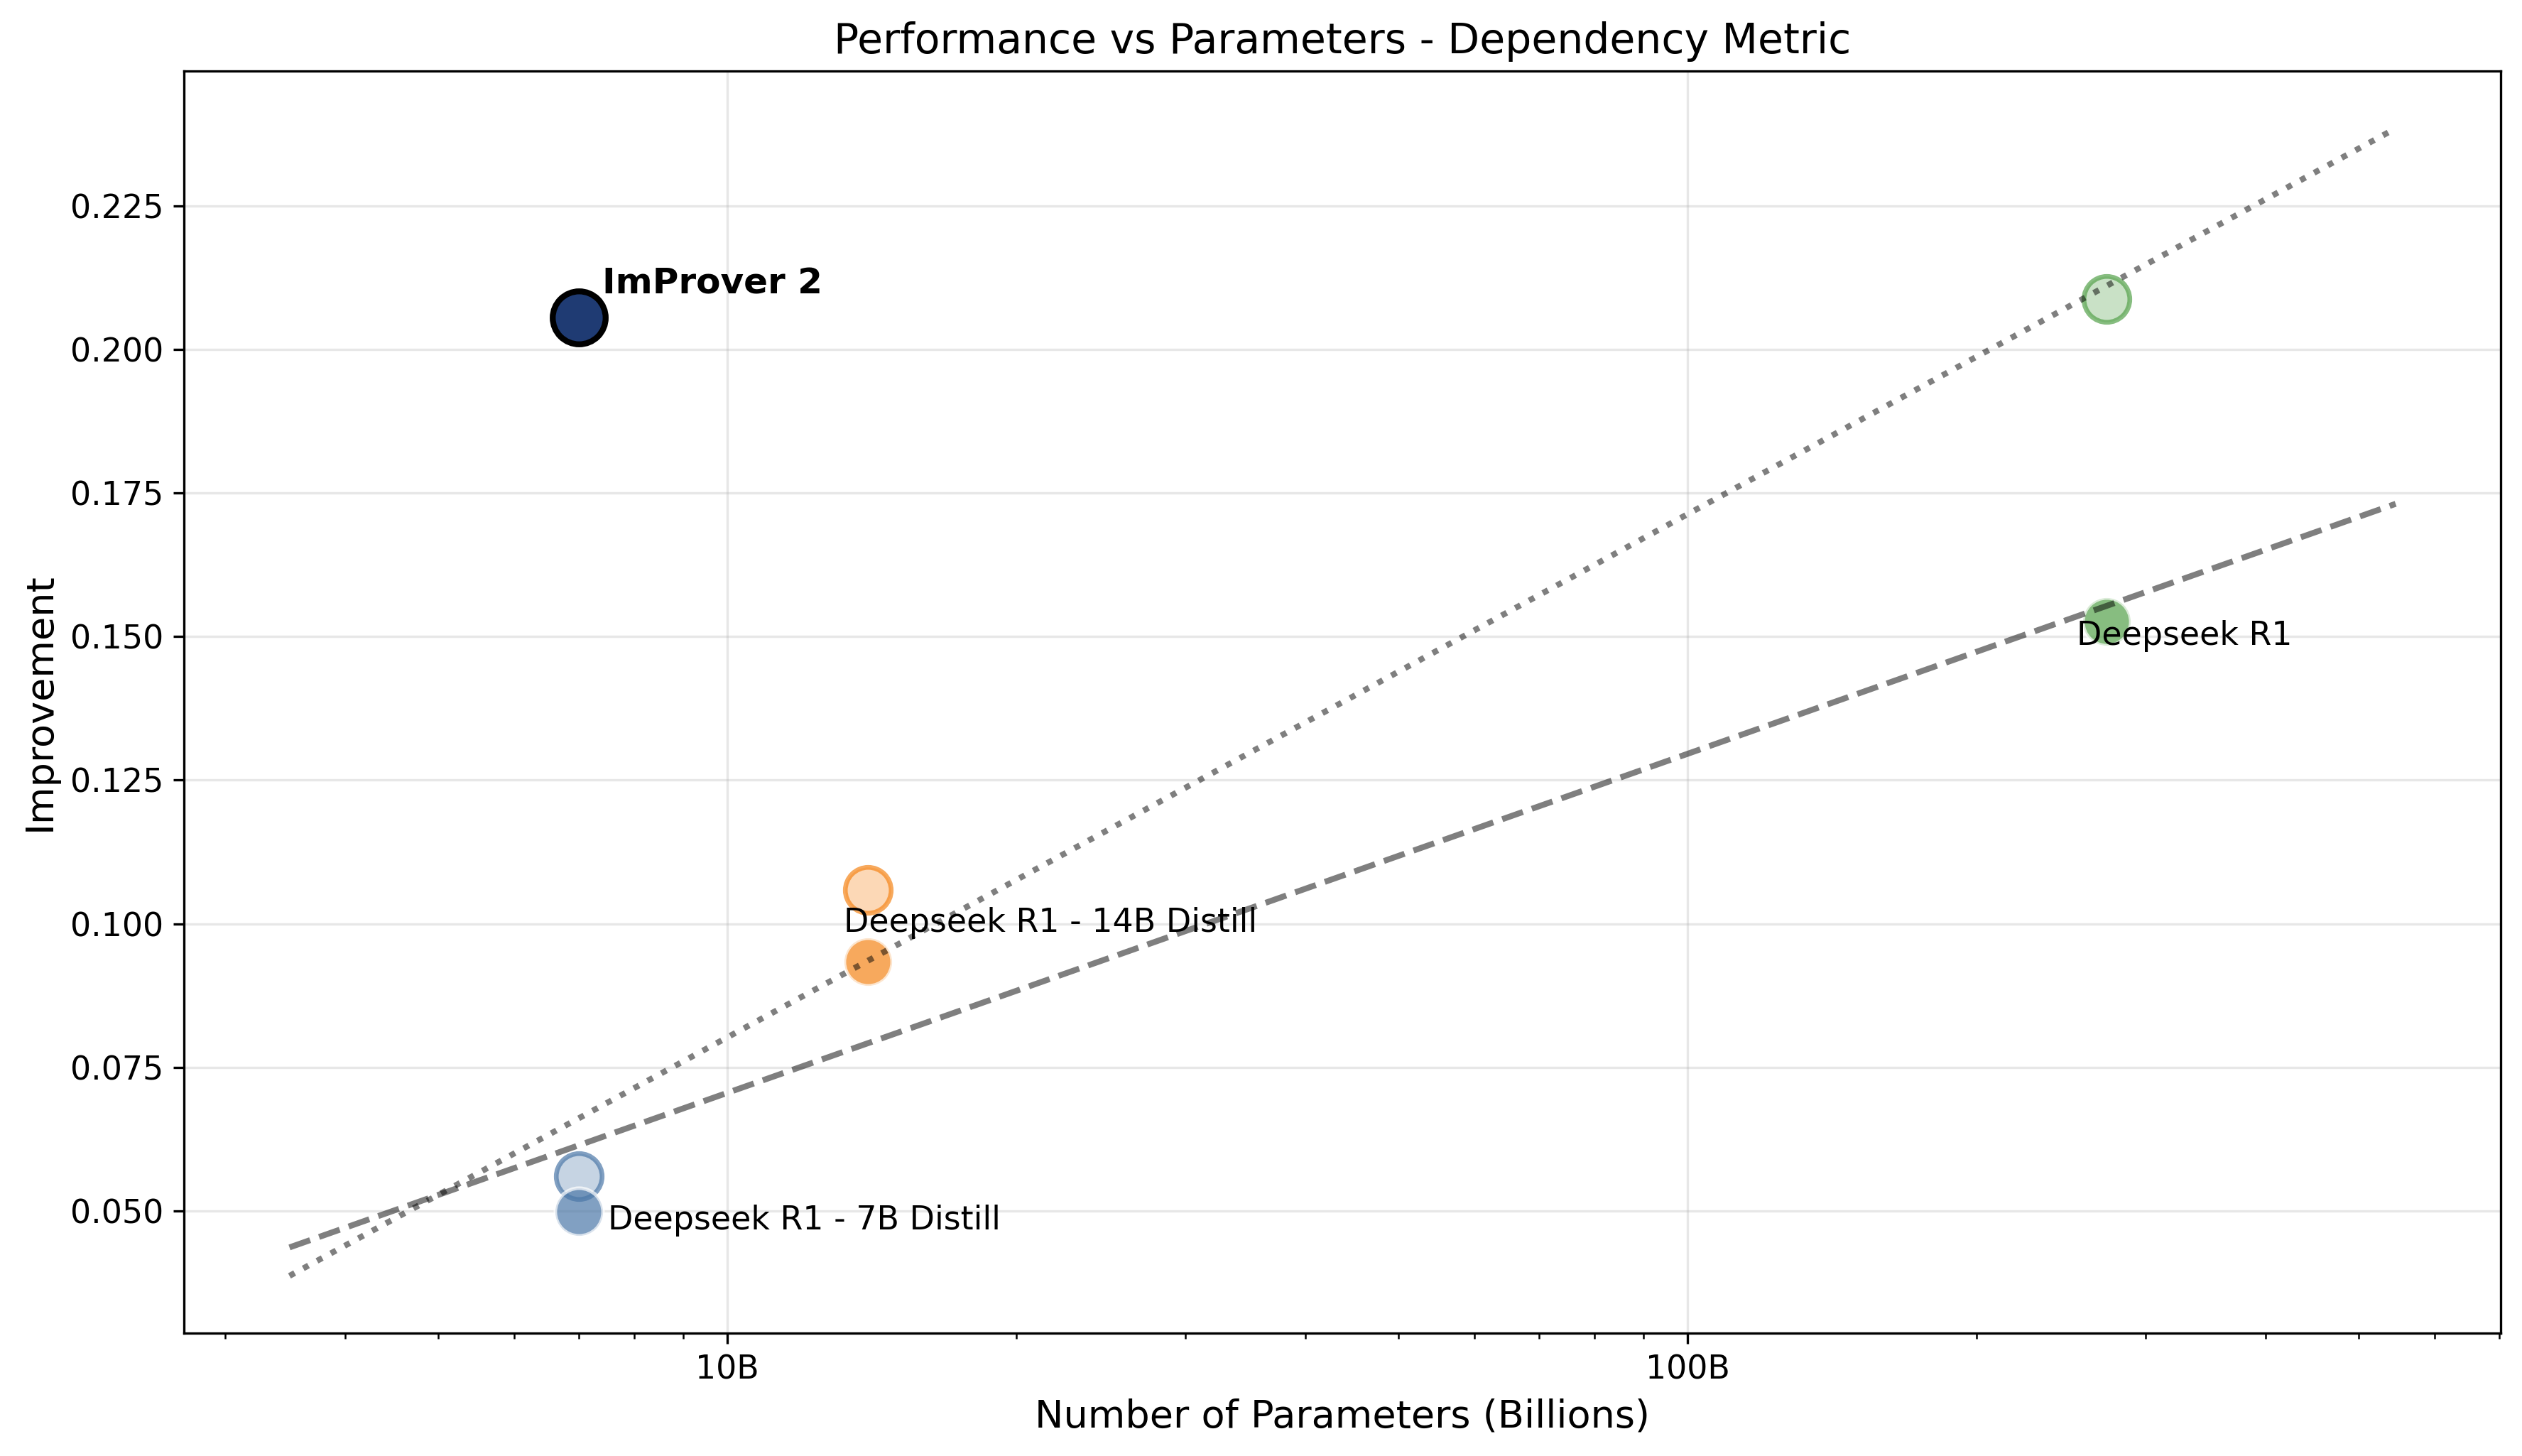
\includegraphics[width=1\linewidth]{figures/Dependency/dependency_param_perf.png}
    
\end{minipage}
\hfill

\begin{minipage}{0.49\linewidth}
    \centering
    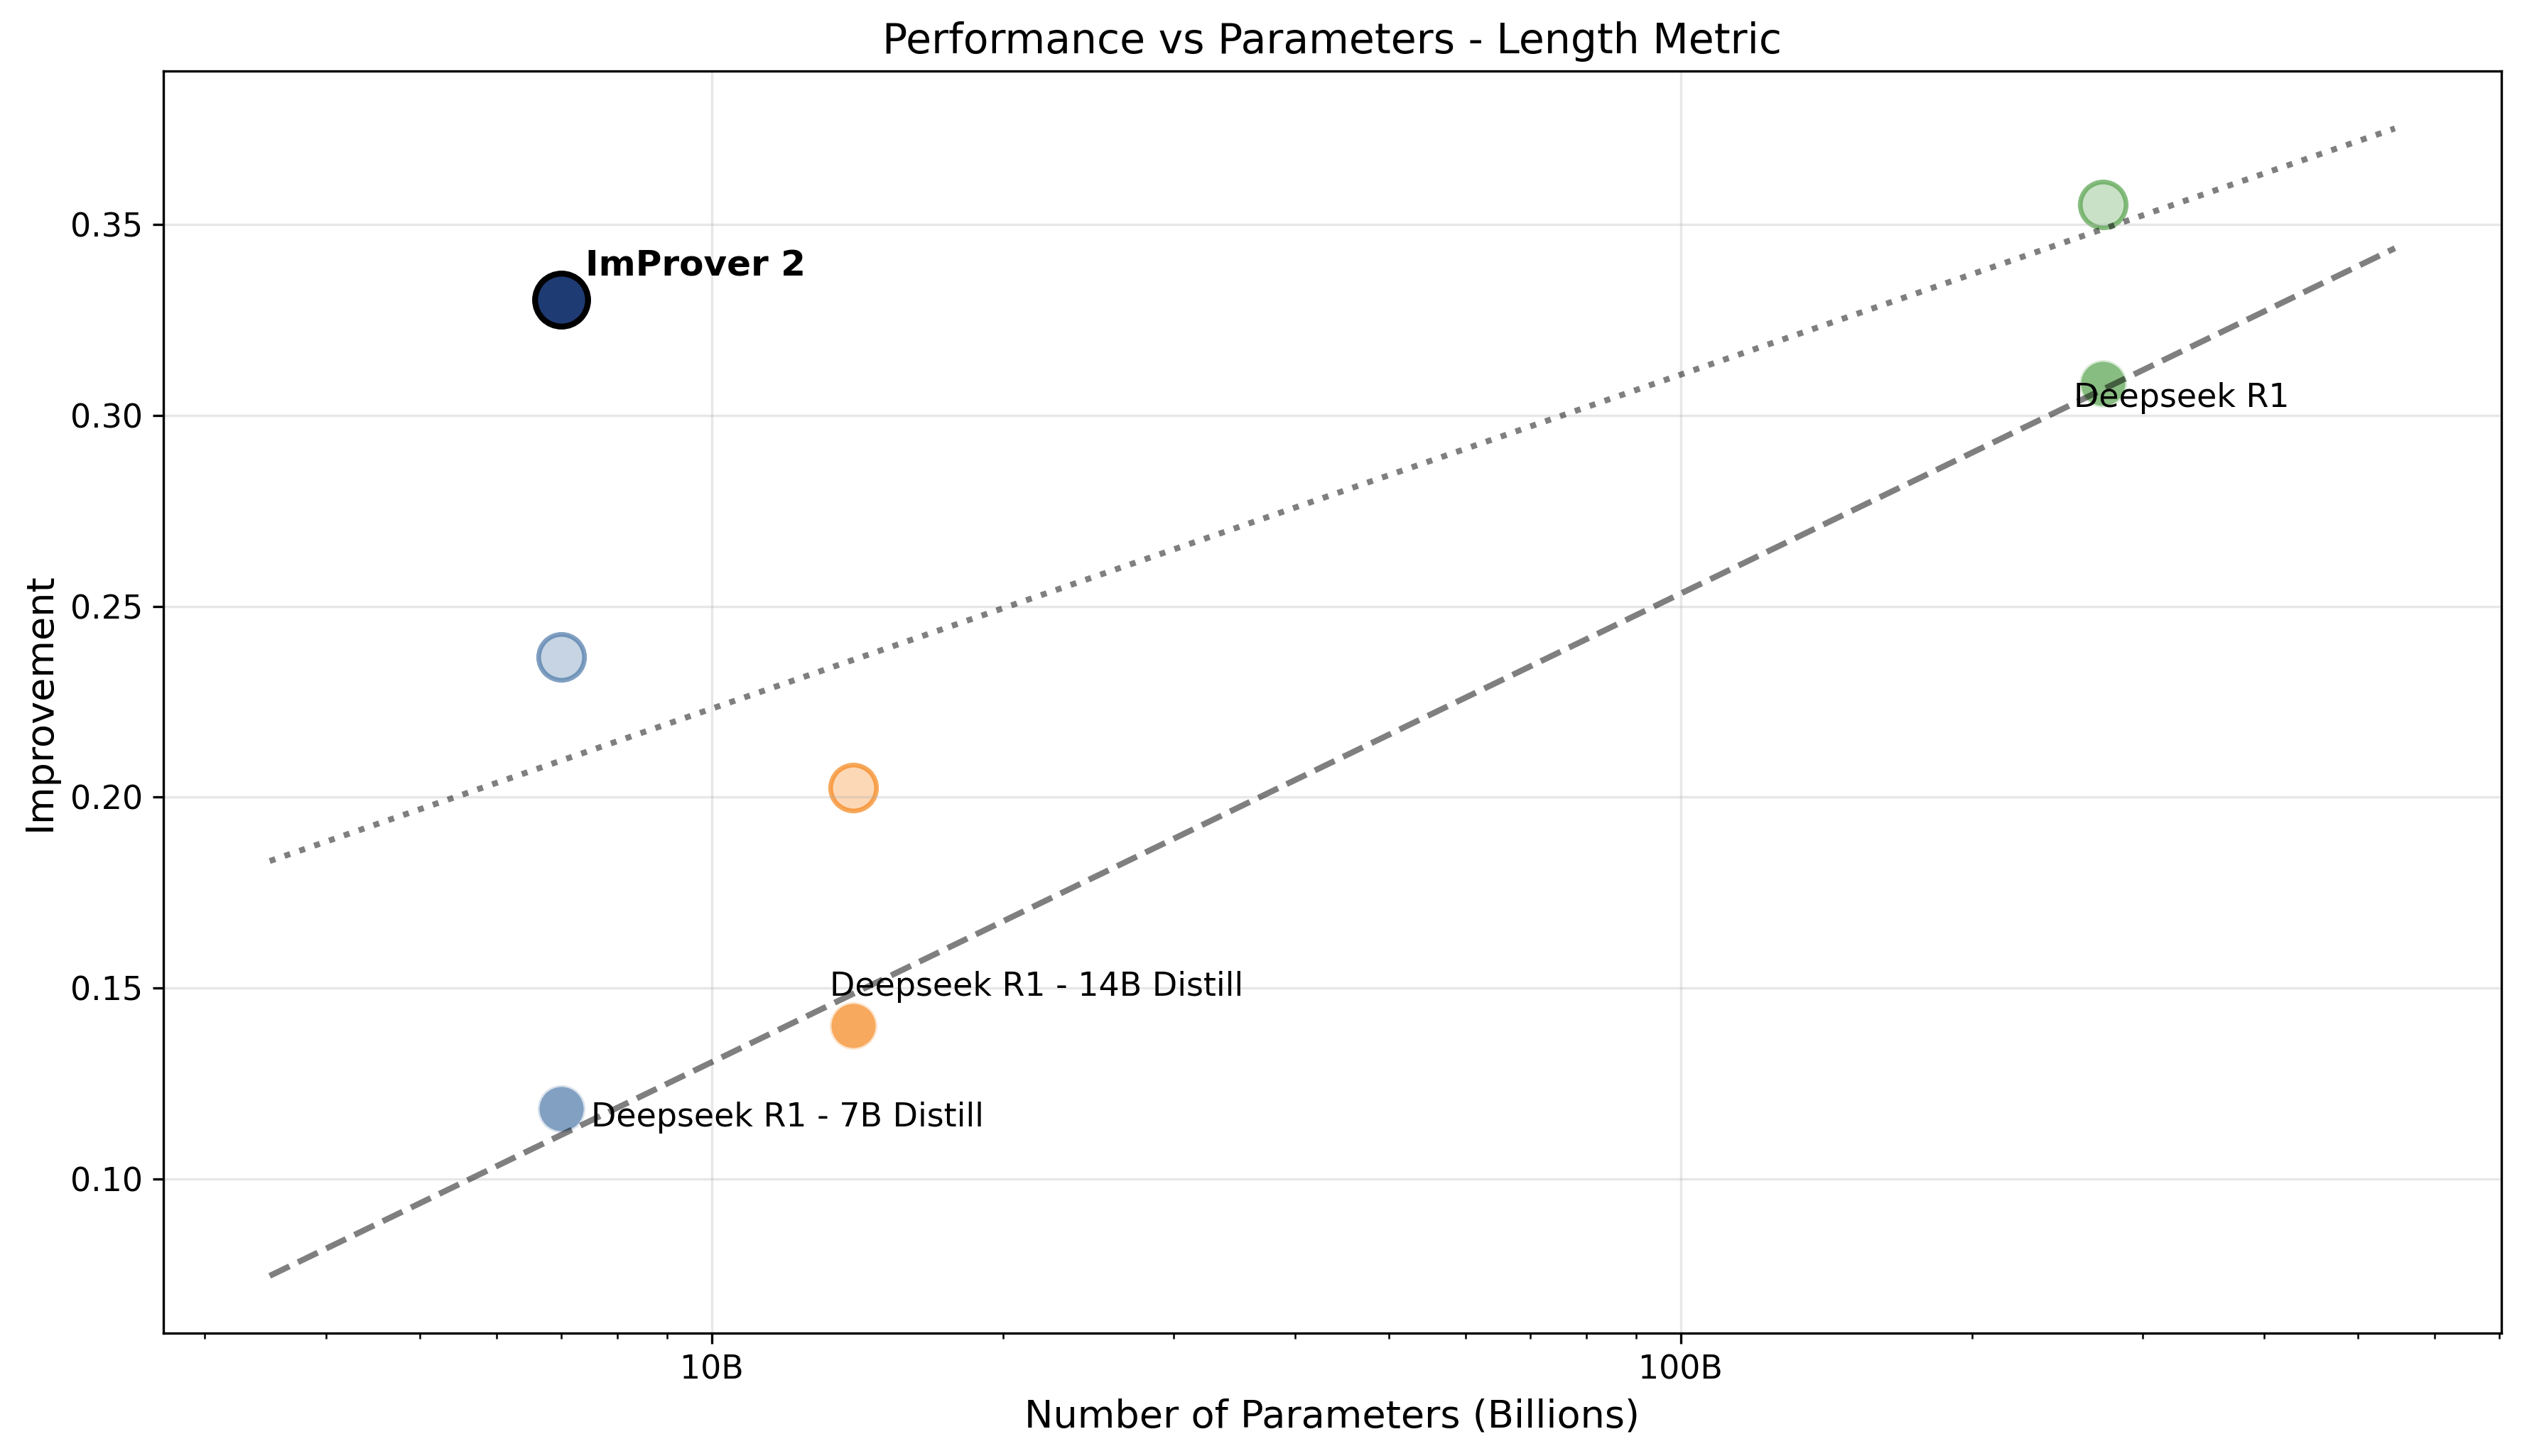
\includegraphics[width=1\linewidth]{figures/Length/length_param_perf.png}
    
    \end{minipage}
        \caption{Effect of parameter count on model performance on mean improvement at best@16 across all three metrics, with ImProver 2 \ marked.}
        \label{fig:param_perf}
\end{figure*}




\subsection{Comparison to Frontier and Prior Systems}
\label{sec:frontier_comparison}


We compare ImProver 2\ against frontier closed-source models, a large open-weight baseline, and the prior \texttt{ImProver} system.
The resulting picture is mixed but informative: frontier systems are already strong proof rewriters, yet their strengths differ by objective, while ImProver 2\ is most competitive on the structural metrics.

Among the frontier baselines evaluated without scaffolding, ImProver 2\ achieves the strongest modularity score ($0.143$), demonstrating that iterative task-specific training surpasses generalist frontier models on the modularity objective, even at much larger parameter counts. On dependency, ImProver 2\ ($0.206$) is competitive with the strongest frontier model evaluated, \texttt{GPT-5-high} ($0.208$), and leads \texttt{GPT-5-mini} ($0.203$); we treat all three as effectively tied at the level of mean performance. On length, ImProver 2\ ($0.330$) matches \texttt{GPT-5-mini} and exceeds \texttt{GPT-oss-120B} ($0.321$), trailing only \texttt{GPT-5-high} ($0.660$), which represents a qualitatively different operating point in terms of inference cost.

% Relative to large open-weight baselines, ImProver 2\ is also strong.
% It matches or exceeds \texttt{GPT-oss-120B} on both length and dependency despite starting from a much smaller base model, suggesting that metric-specific self-improvement can recover a substantial fraction of the gains otherwise obtained through scale.


\begin{figure*}
    \centering
    
\begin{minipage}{0.49\linewidth}
    \centering
    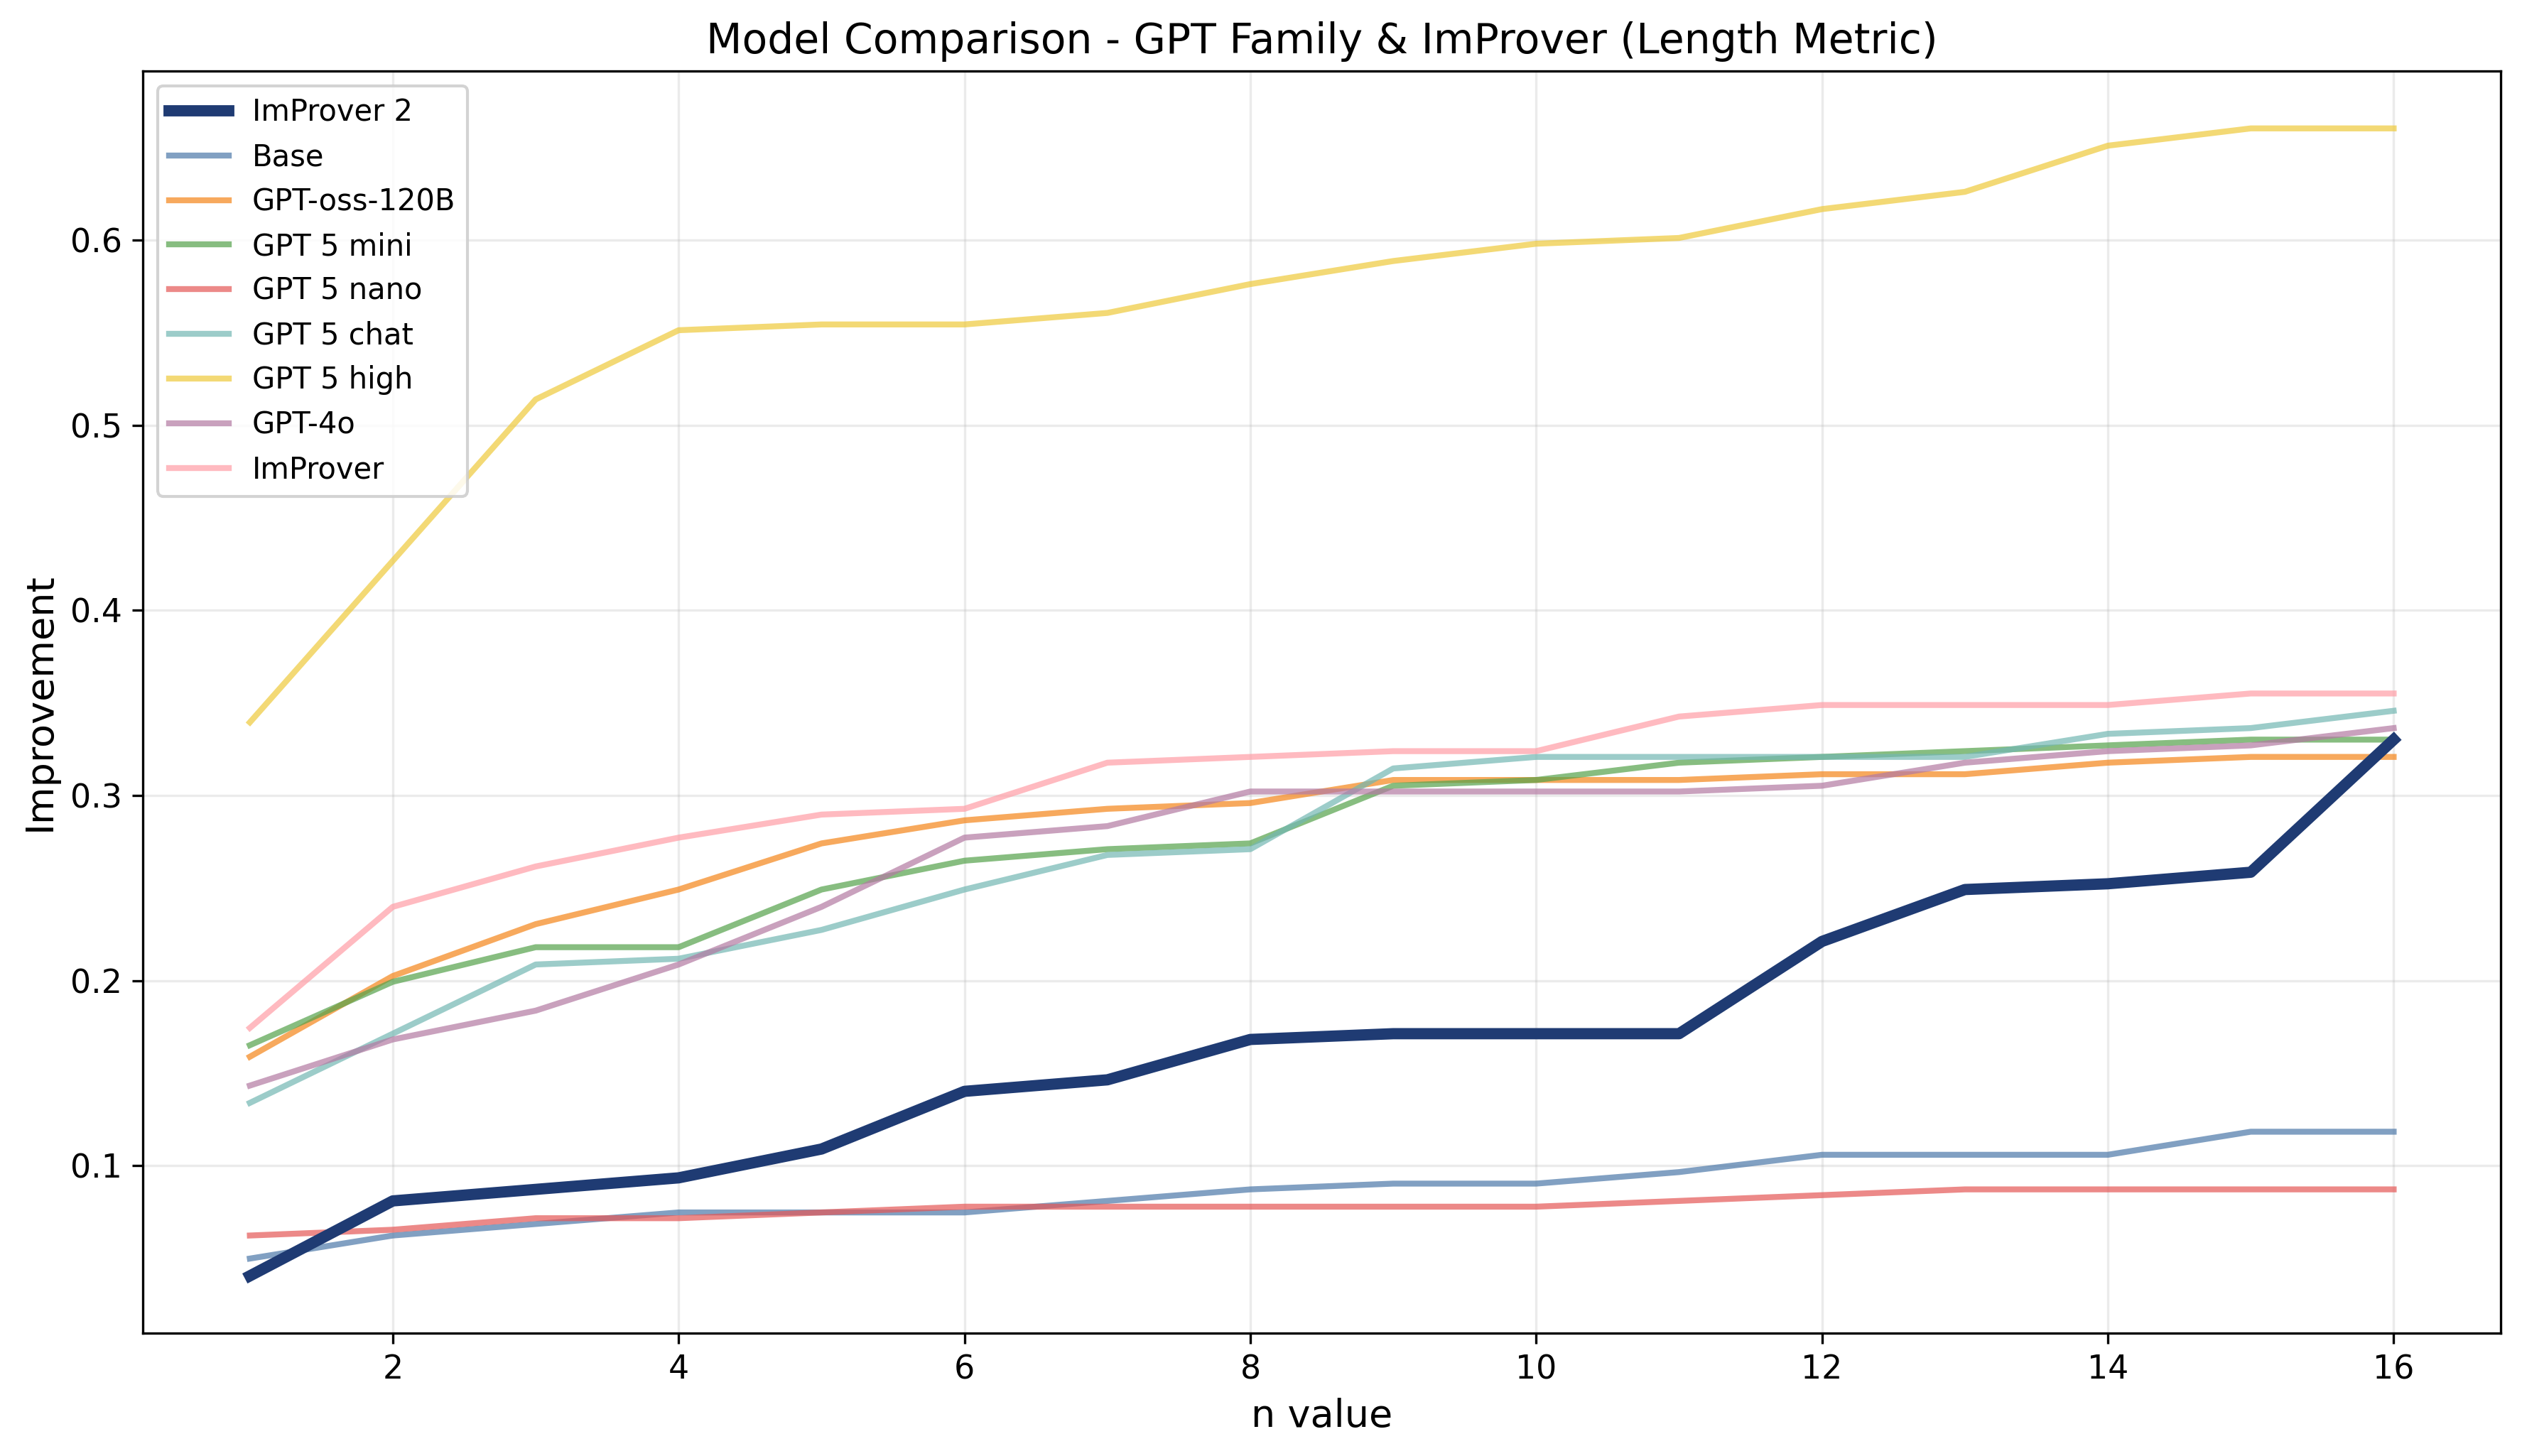
\includegraphics[width=1\linewidth]{figures/Length/length_gpt_improver_comparison.png}
    \label{fig:length_gpt_improver_comparison}
\end{minipage}
\hfill
\begin{minipage}{0.49\linewidth}
    \centering
    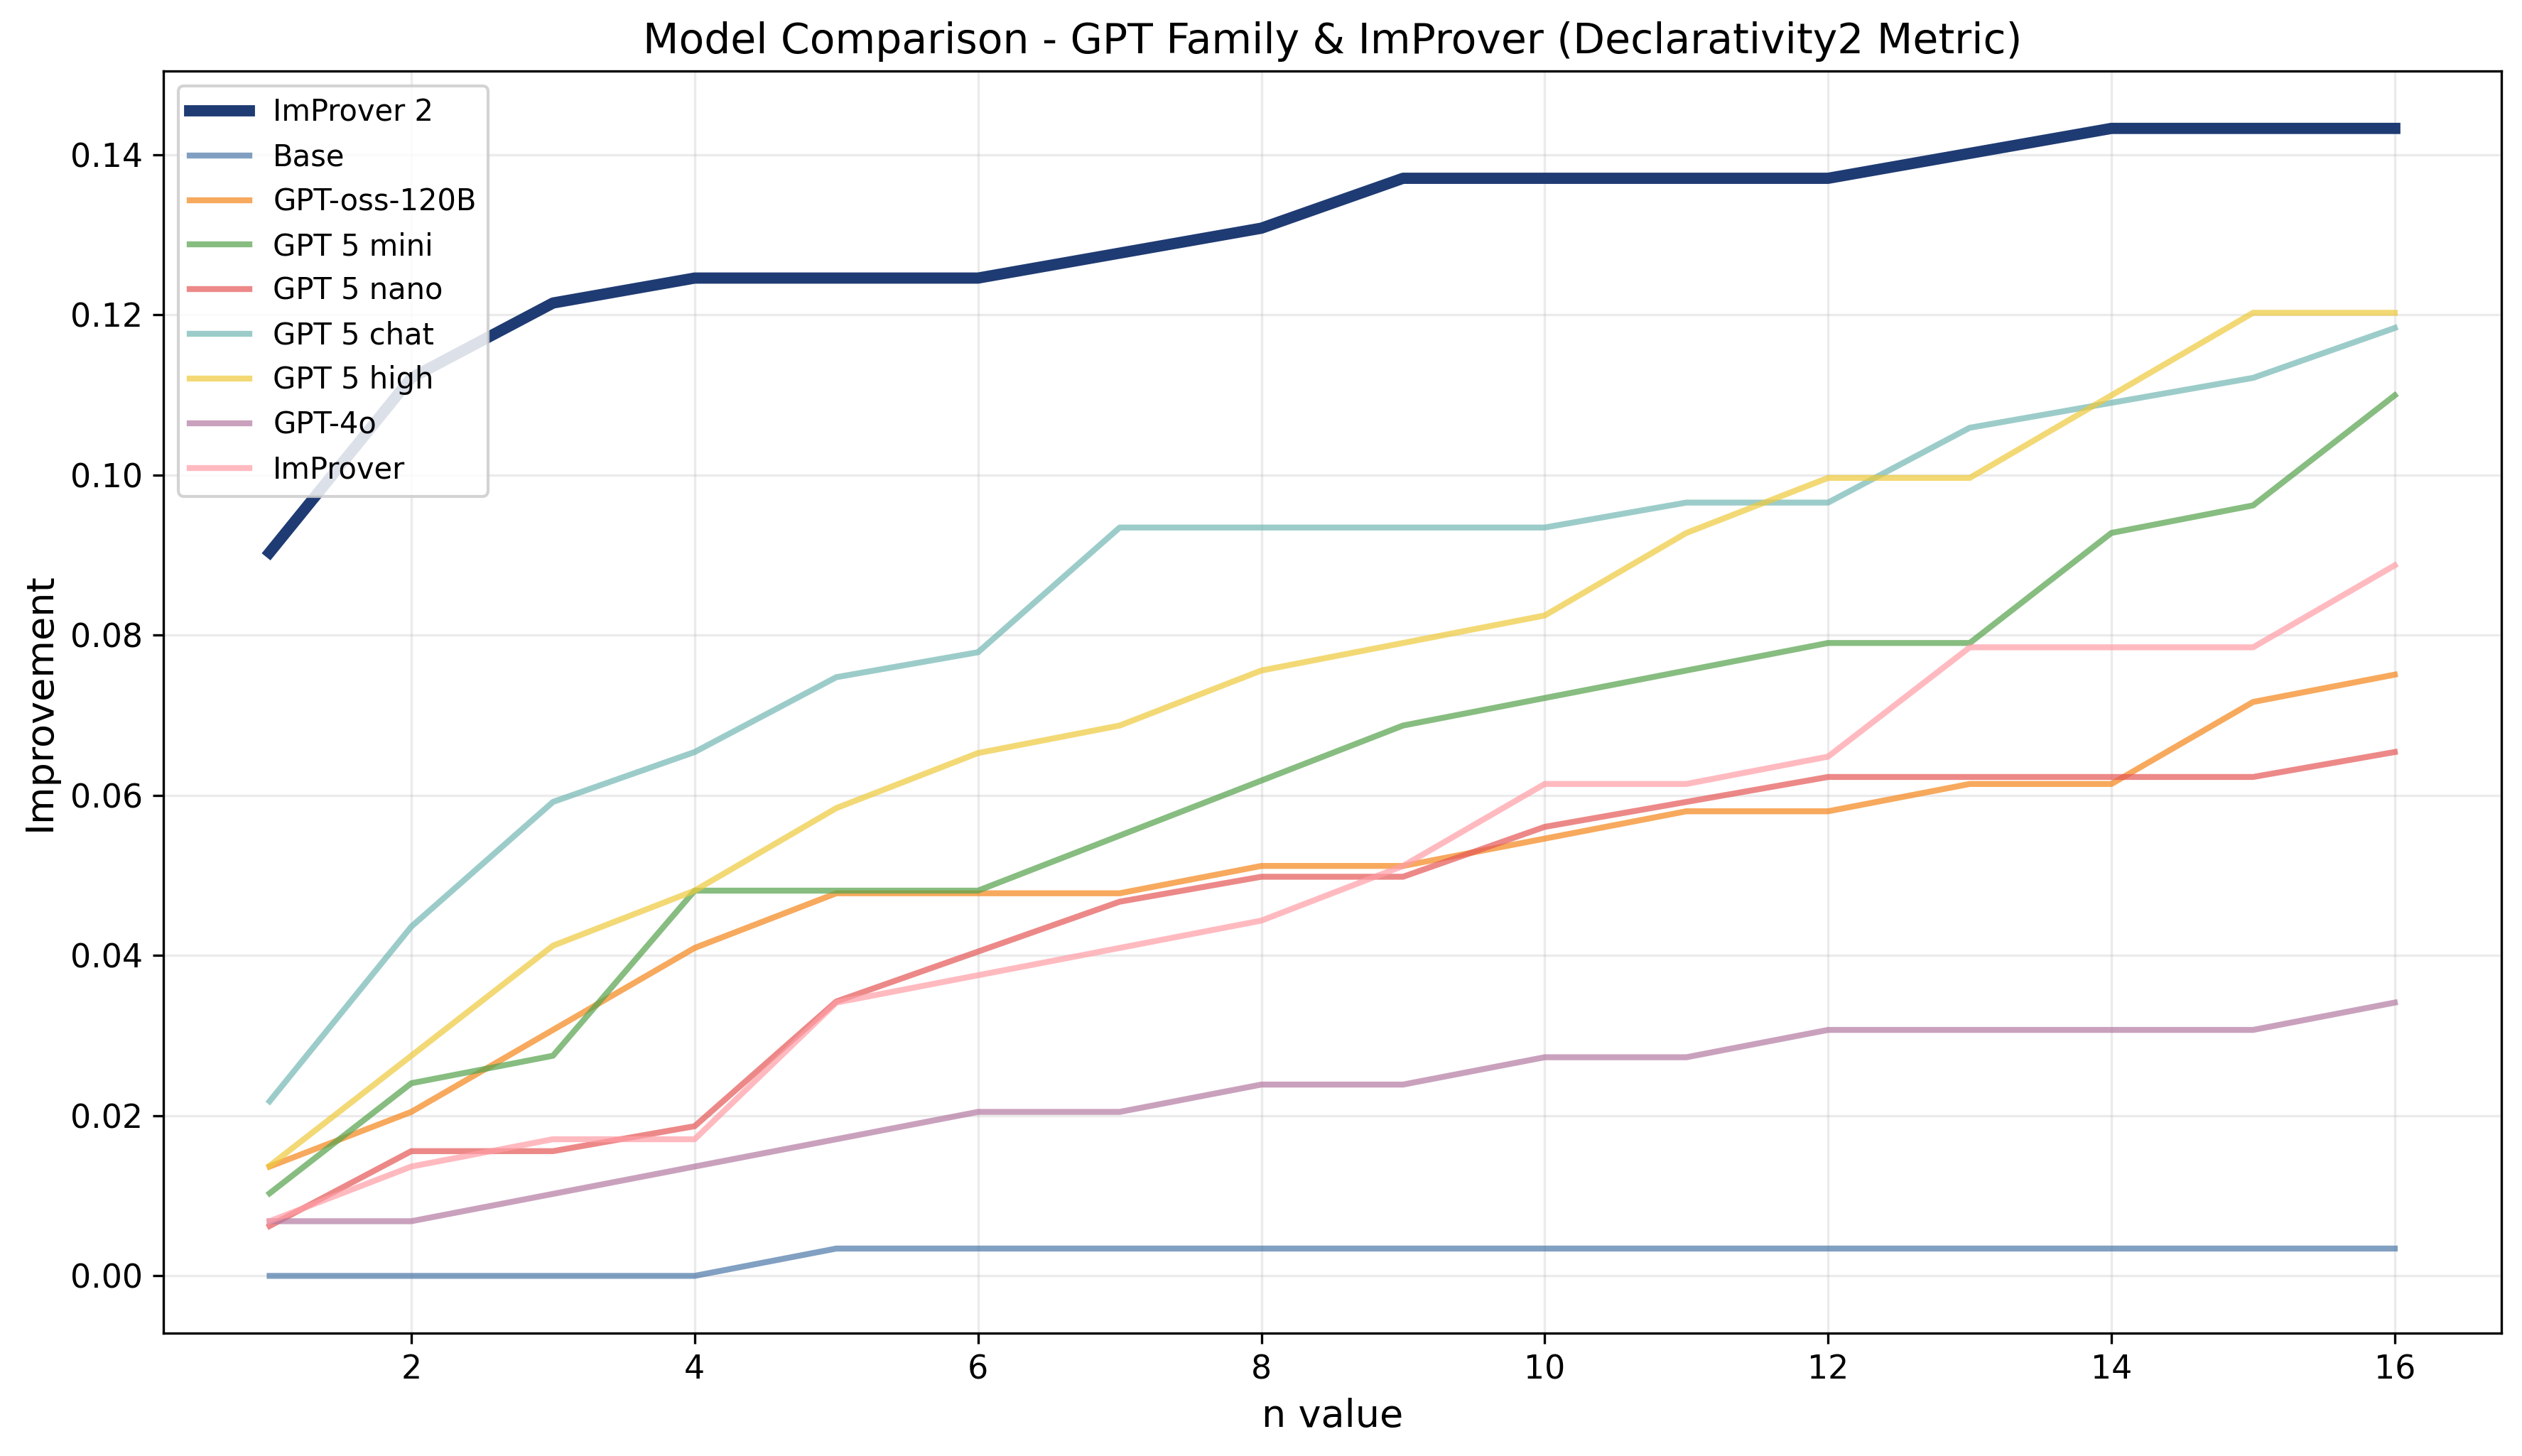
\includegraphics[width=1\linewidth]{figures/Modularity/declarativity2_gpt_improver_comparison.png}
    \label{fig:declarativity2_gpt_improver_comparison}
\end{minipage}
\hfill
\begin{minipage}{0.49\linewidth}
    \centering
    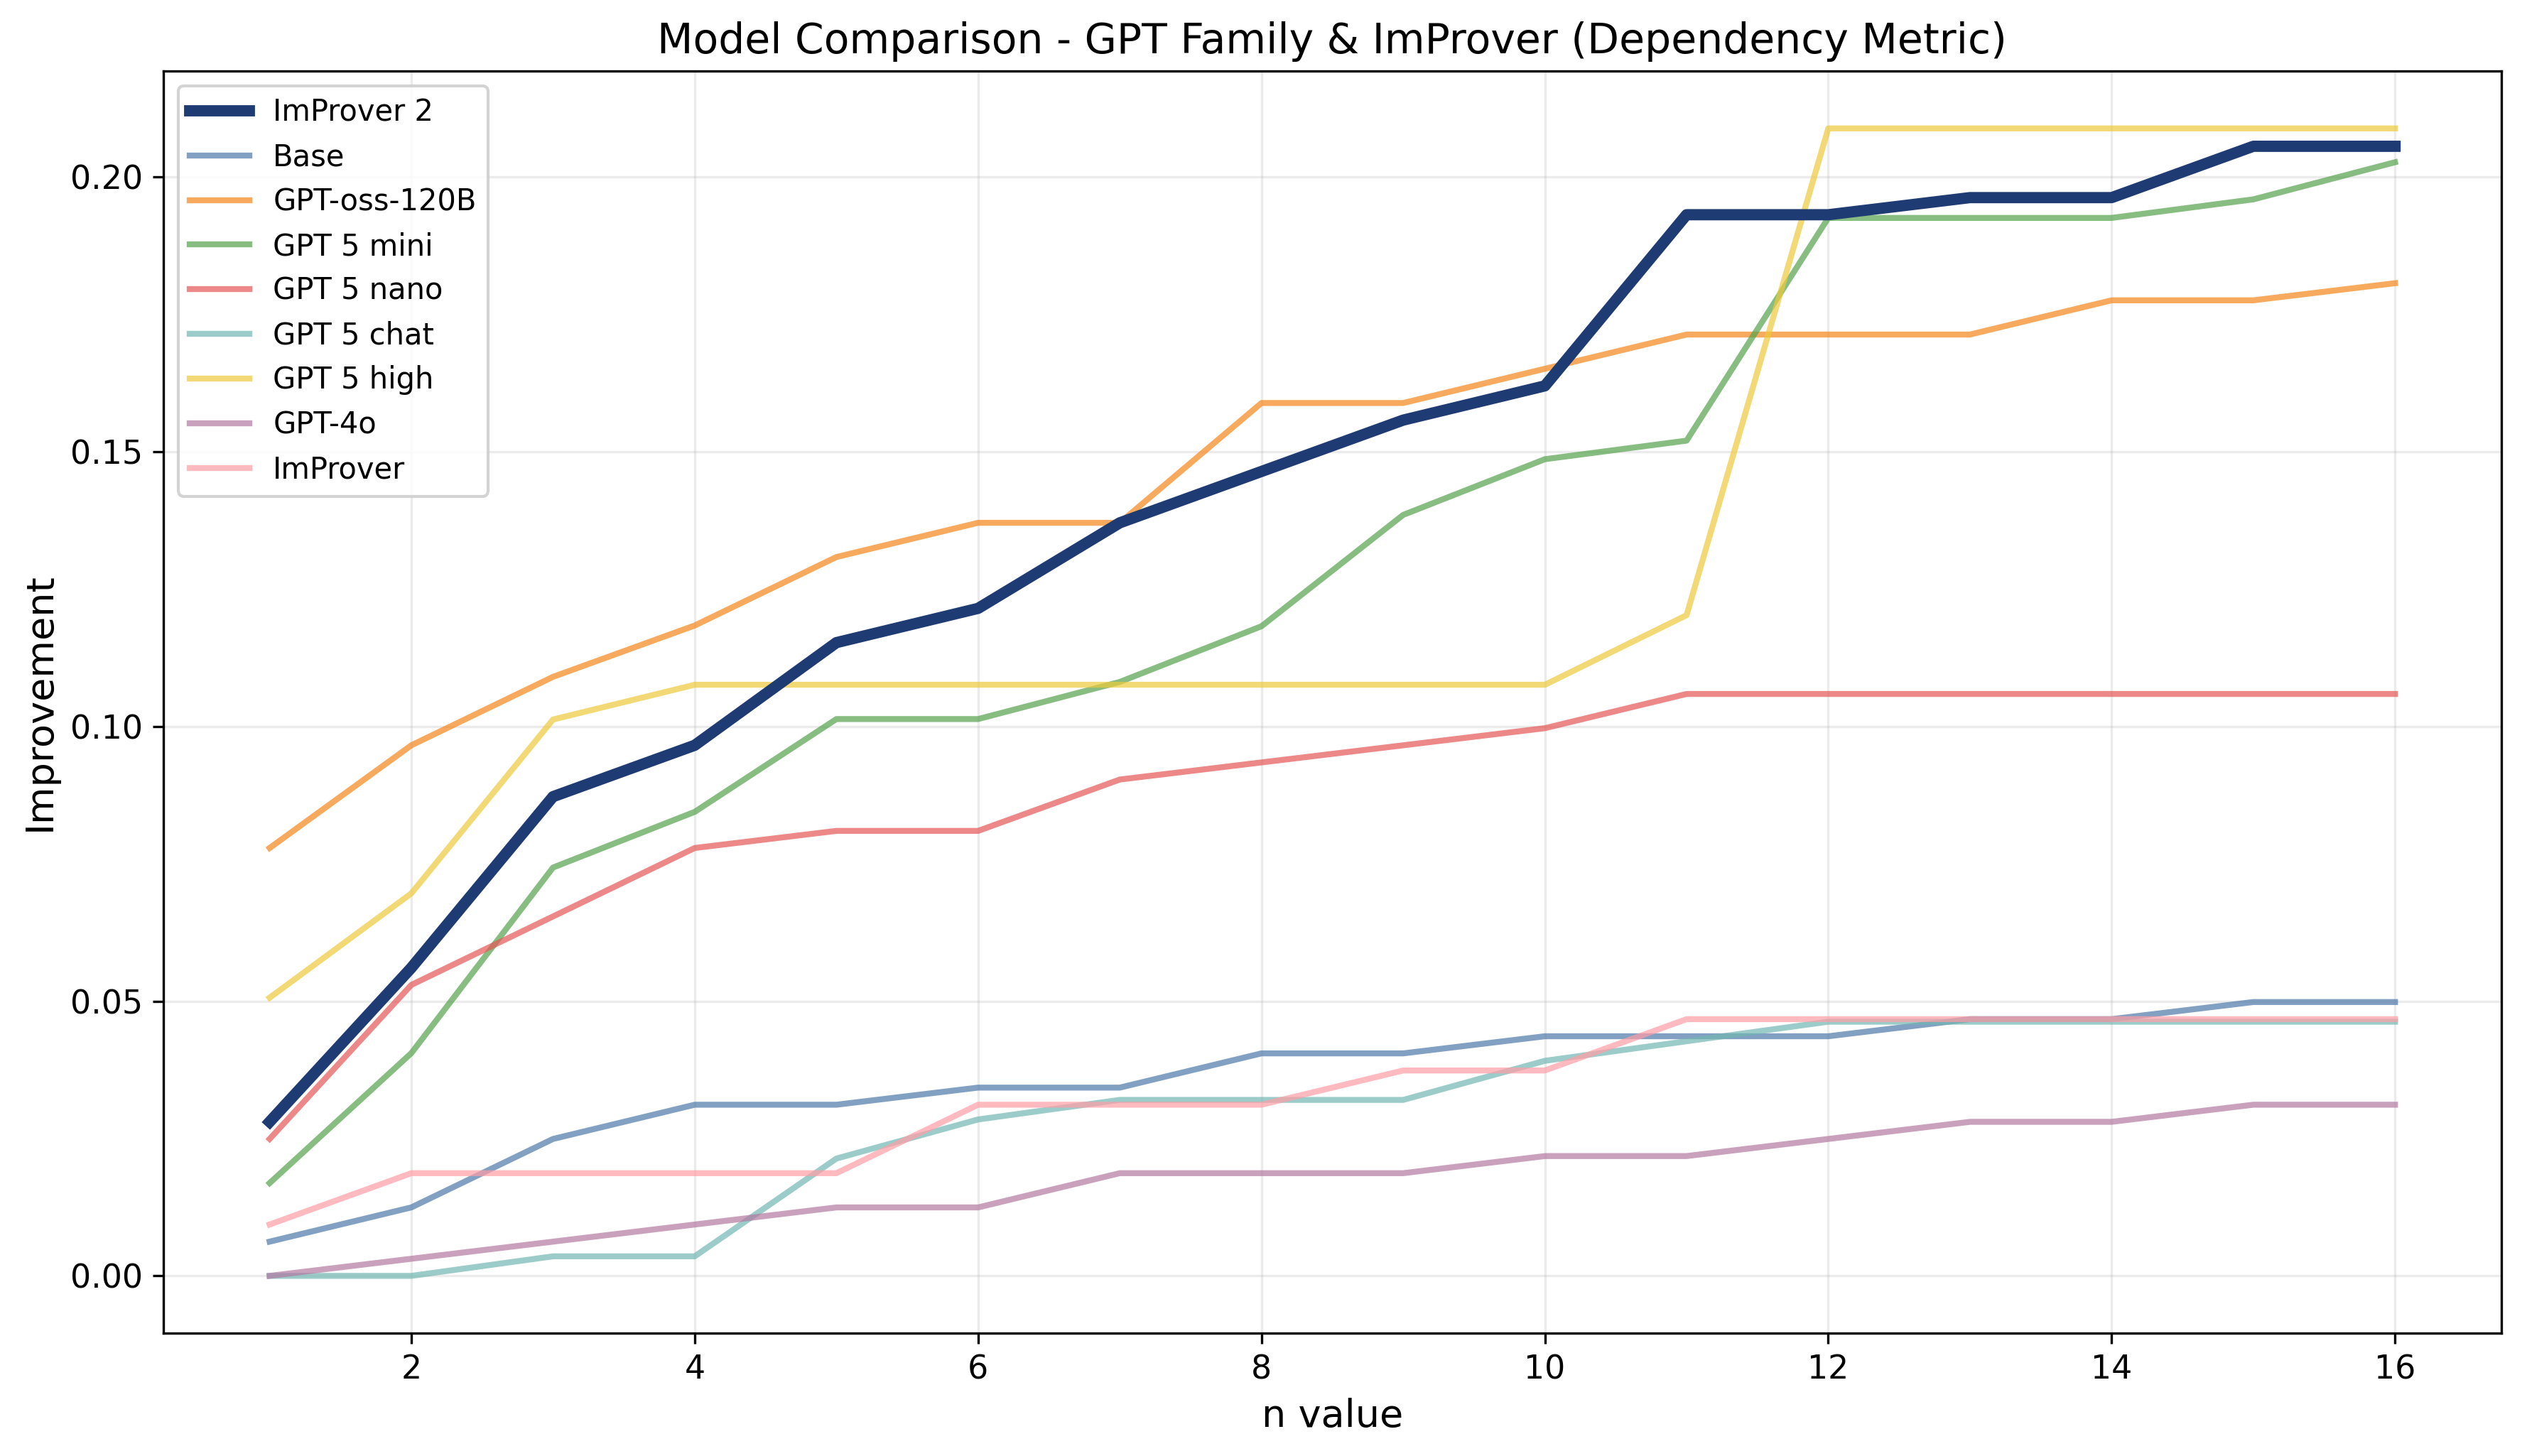
\includegraphics[width=1\linewidth]{figures/Dependency/dependency_gpt_improver_comparison.png}
    \label{fig:dependency_gpt_improver_comparison}
    \end{minipage}
    \caption{Comparison of ImProver 2 \ against frontier GPT-based models and ImProver, evaluated on mean improvement at best@$n$ on all metrics, from $n=1$ to $n=16$.}
        \label{fig:gpt_improver_comparison}

\end{figure*}



Relative to large open-weight baselines, ImProver 2\ is also strong.
It matches or exceeds \texttt{GPT-oss-120B} on all three metrics despite starting 
from a much smaller base model. We note that \texttt{GPT-oss-120B} is a sparse 
mixture-of-experts model activating approximately 5B parameters per token, so the 
raw parameter count comparison overstates the computational gap; nonetheless, \texttt{GPT-oss-120B} is a significantly more powerful base model compared to the \texttt{DeepSeek-R1-Distill-Qwen-7B} base that is used by ImProver 2 (as shown by the comparative evaluation of \cite{openai2025gptoss120bgptoss20bmodel},\cite{DeepseekR1}). As such, these results demonstrate that metric-specific iterative self-improvement can substitute for large increases in both parameter count and base model capability for this task.

The comparison with the prior \texttt{ImProver} system is also revealing. The original ImProver system leads ImProver 2\ on length ($0.355$ vs.\ $0.330$), consistent 
with its use of an agentic prompting strategy with a strong proprietary base model. By contrast, ImProver 2\ leads on modularity ($0.143$ vs.\ $0.088$) and outperforms ImProver substantially on dependency ($0.206$ vs.\ $0.047$), demonstrating that on these more complex metrics, iterative structural supervision learns refactoring capabilities that agentic prompting alone does not reliably acquire.



\subsection{Effect of Neurosymbolic Scaffolding}
\label{sec:scaffold_power}
\begin{table*}[t]
\centering
\caption{\textbf{Scaffold Evaluations.} Effect of neurosymbolic scaffolding. Mean improvement at best@16 with and without the scaffold $\Psi$, across model families and metrics.}
\small
\setlength{\tabcolsep}{4pt}
\resizebox{\textwidth}{!}{%
\begin{tabular}{llccccccccc}
\toprule
\textbf{Metric} & \textbf{Variant} & \textbf{DS-R1 7B} & \textbf{DS-R1 14B} & \textbf{DS-R1 671B} & \textbf{GPT-4o} & \textbf{GPT-oss-120B} & \textbf{GPT-5-nano} & \textbf{GPT-5-mini} & \textbf{GPT-5-chat} & \textbf{GPT-5-high} \\
\midrule
\multirow{2}{*}{Length}
  & Base     & 0.118 & 0.140 & 0.308 & 0.336 & 0.321 & 0.087 & 0.330 & 0.346 & 0.660 \\
  & Scaffold & \textbf{0.236} & \textbf{0.202} & \textbf{0.355} & \textbf{0.396} & \textbf{0.508} & \textbf{0.296} & \textbf{0.632} & \textbf{0.576} & \textbf{0.875} \\
\midrule
\multirow{2}{*}{Mod.}
  & Base     & 0.003 & \textbf{0.037} & 0.055 & 0.034 & 0.075 & 0.065 & 0.109 & 0.118 & 0.120 \\
  & Scaffold & \textbf{0.007} & 0.024 & \textbf{0.100} & \textbf{0.092} & \textbf{0.092} & \textbf{0.069} & \textbf{0.123} & \textbf{0.153} & \textbf{--} \\
\midrule
\multirow{2}{*}{Dep.}
  & Base     & 0.050 & 0.093 & 0.153 & 0.050 & 0.181 & 0.106 & 0.203 & 0.046 & 0.208 \\
  & Scaffold & \textbf{0.056} & \textbf{0.106} & \textbf{0.209} & \textbf{0.075} & \textbf{0.406} & \textbf{0.108} & \textbf{0.267} & \textbf{0.087} & \textbf{0.315} \\
\bottomrule
\end{tabular}%
}
\label{tab:scaffold}
\end{table*}
% \begin{table}[t]
% \centering
% \caption{\textbf{Scaffold Evaluations.} Effect of neurosymbolic scaffolding. Mean improvement at best@16 with and without the scaffold $\Psi$, across model families and metrics.}
% \small
% \setlength{\tabcolsep}{6pt}
% \begin{tabular}{llcc}
% \toprule
% \textbf{Model} & \textbf{Metric} & \textbf{Base} & \textbf{Scaffold} \\
% \midrule
% \multirow{3}{*}{DeepSeek-R1 7B}
%   & Length & 0.118 & \textbf{0.236} \\
%   & Mod.   & 0.003 & \textbf{0.007} \\
%   & Dep.   & 0.050 &\textbf{ 0.056} \\
% \midrule
% \multirow{3}{*}{DeepSeek-R1 14B}
%   & Length & 0.140 & \textbf{0.202} \\
%   & Mod.   & \textbf{0.037} & 0.024 \\
%   & Dep.   & 0.093 & \textbf{0.106} \\
% \midrule
% \multirow{3}{*}{DeepSeek-R1 (671B)}
%   & Length & 0.308 & \textbf{0.355} \\
%   & Mod.   & 0.055 & \textbf{0.100} \\
%   & Dep.   & 0.153 & \textbf{0.209} \\
% \midrule
% \multirow{3}{*}{GPT-4o}
%   & Length & 0.336 & \textbf{0.396} \\
%   & Mod.   & 0.034 & \textbf{0.092} \\
%   & Dep.   & 0.050 & \textbf{0.075} \\
% \midrule
% \multirow{3}{*}{GPT-oss-120B}
%   & Length & 0.321 & \textbf{0.508} \\
%   & Mod.   & 0.075 & \textbf{0.092} \\
%   & Dep.   & 0.181 & \textbf{0.406} \\
% \midrule
% \multirow{3}{*}{GPT-5-nano}
%   & Length & 0.087 & \textbf{0.296} \\
%   & Mod.   & 0.065 & \textbf{0.069} \\
%   & Dep.   & 0.106 & \textbf{0.108} \\
% \midrule
% \multirow{3}{*}{GPT-5-mini}
%   & Length & 0.330 & \textbf{0.632} \\
%   & Mod.   & 0.109 & \textbf{0.123} \\
%   & Dep.   & 0.203 & \textbf{0.267} \\
% \midrule
% \multirow{3}{*}{GPT-5-chat}
%   & Length & 0.346 & \textbf{0.576} \\
%   & Mod.   & 0.118 & \textbf{0.153} \\
%   & Dep.   & 0.046 & \textbf{0.087} \\
% \midrule
% \multirow{3}{*}{GPT-5-high}
%   & Length & 0.660 & \textbf{0.875} \\
%   & Mod.   & 0.120 & \textbf{-} \\
%   & Dep.   & 0.208 & \textbf{0.315} \\
% \bottomrule
% \end{tabular}
% \label{tab:scaffold}
% \end{table}


A central claim of this work is that proof optimization is limited not only by model size, but by how well the model is conditioned on the structure of the formal task.
Table~\ref{tab:scaffold} strongly supports this claim.
Across nearly all evaluated generators and metrics, adding the scaffold $\Psi$ improves mean best@16 performance, often by a large margin.

The effect is especially striking on length.
For \texttt{DeepSeek-R1 7B}, scaffolding nearly doubles performance from $0.118$ to $0.236$ even before iterative training.
For stronger frontier models the gains are larger still in absolute terms: \texttt{GPT-5-mini} rises from $0.330$ to $0.632$, \texttt{GPT-5-chat} from $0.346$ to $0.576$, and \texttt{GPT-oss-120B} from $0.321$ to $0.508$.
This suggests that the scaffold is not merely compensating for weak base models; rather, it changes the representation of the task in a way that makes better rewrites easier to discover under a fixed sampling budget.

This pattern extends even to the strongest evaluated system: \texttt{GPT-5-high} improves from $0.660$ to $0.875$ on length under scaffolding, suggesting that Lean-aware conditioning provides complementary information even to large high-reasoning models.

The dependency metric shows a similar pattern.
Most models benefit substantially from scaffolding, with especially large gains for \texttt{GPT-oss-120B} ($0.181 \to 0.406$), \texttt{GPT-5-mini} ($0.203 \to 0.267$), and \texttt{GPT-5-chat} ($0.046 \to 0.087$).
Modularity gains are smaller and less uniform, but still mostly positive.
The main exception is \texttt{DeepSeek-R1 14B}, where modularity decreases slightly under scaffolding ($0.037 \to 0.024$).
Given the broader pattern across both open and closed models, we view this as an outlier rather than evidence against the scaffold.

Overall, the scaffold appears to expand the set of useful rewrites the model can reliably attempt.
By exposing goal-state information, relevant context, and informal abstractions, it helps both small and large models move beyond surface-level editing toward more substantive proof refactoring by improving models' abilities to search over valid higher-value rewrites under a fixed sampling budget.


\subsection{Training and Iteration}
\label{sec:train}


\begin{figure*}
    \centering

\begin{minipage}{0.49\linewidth}
    \centering
    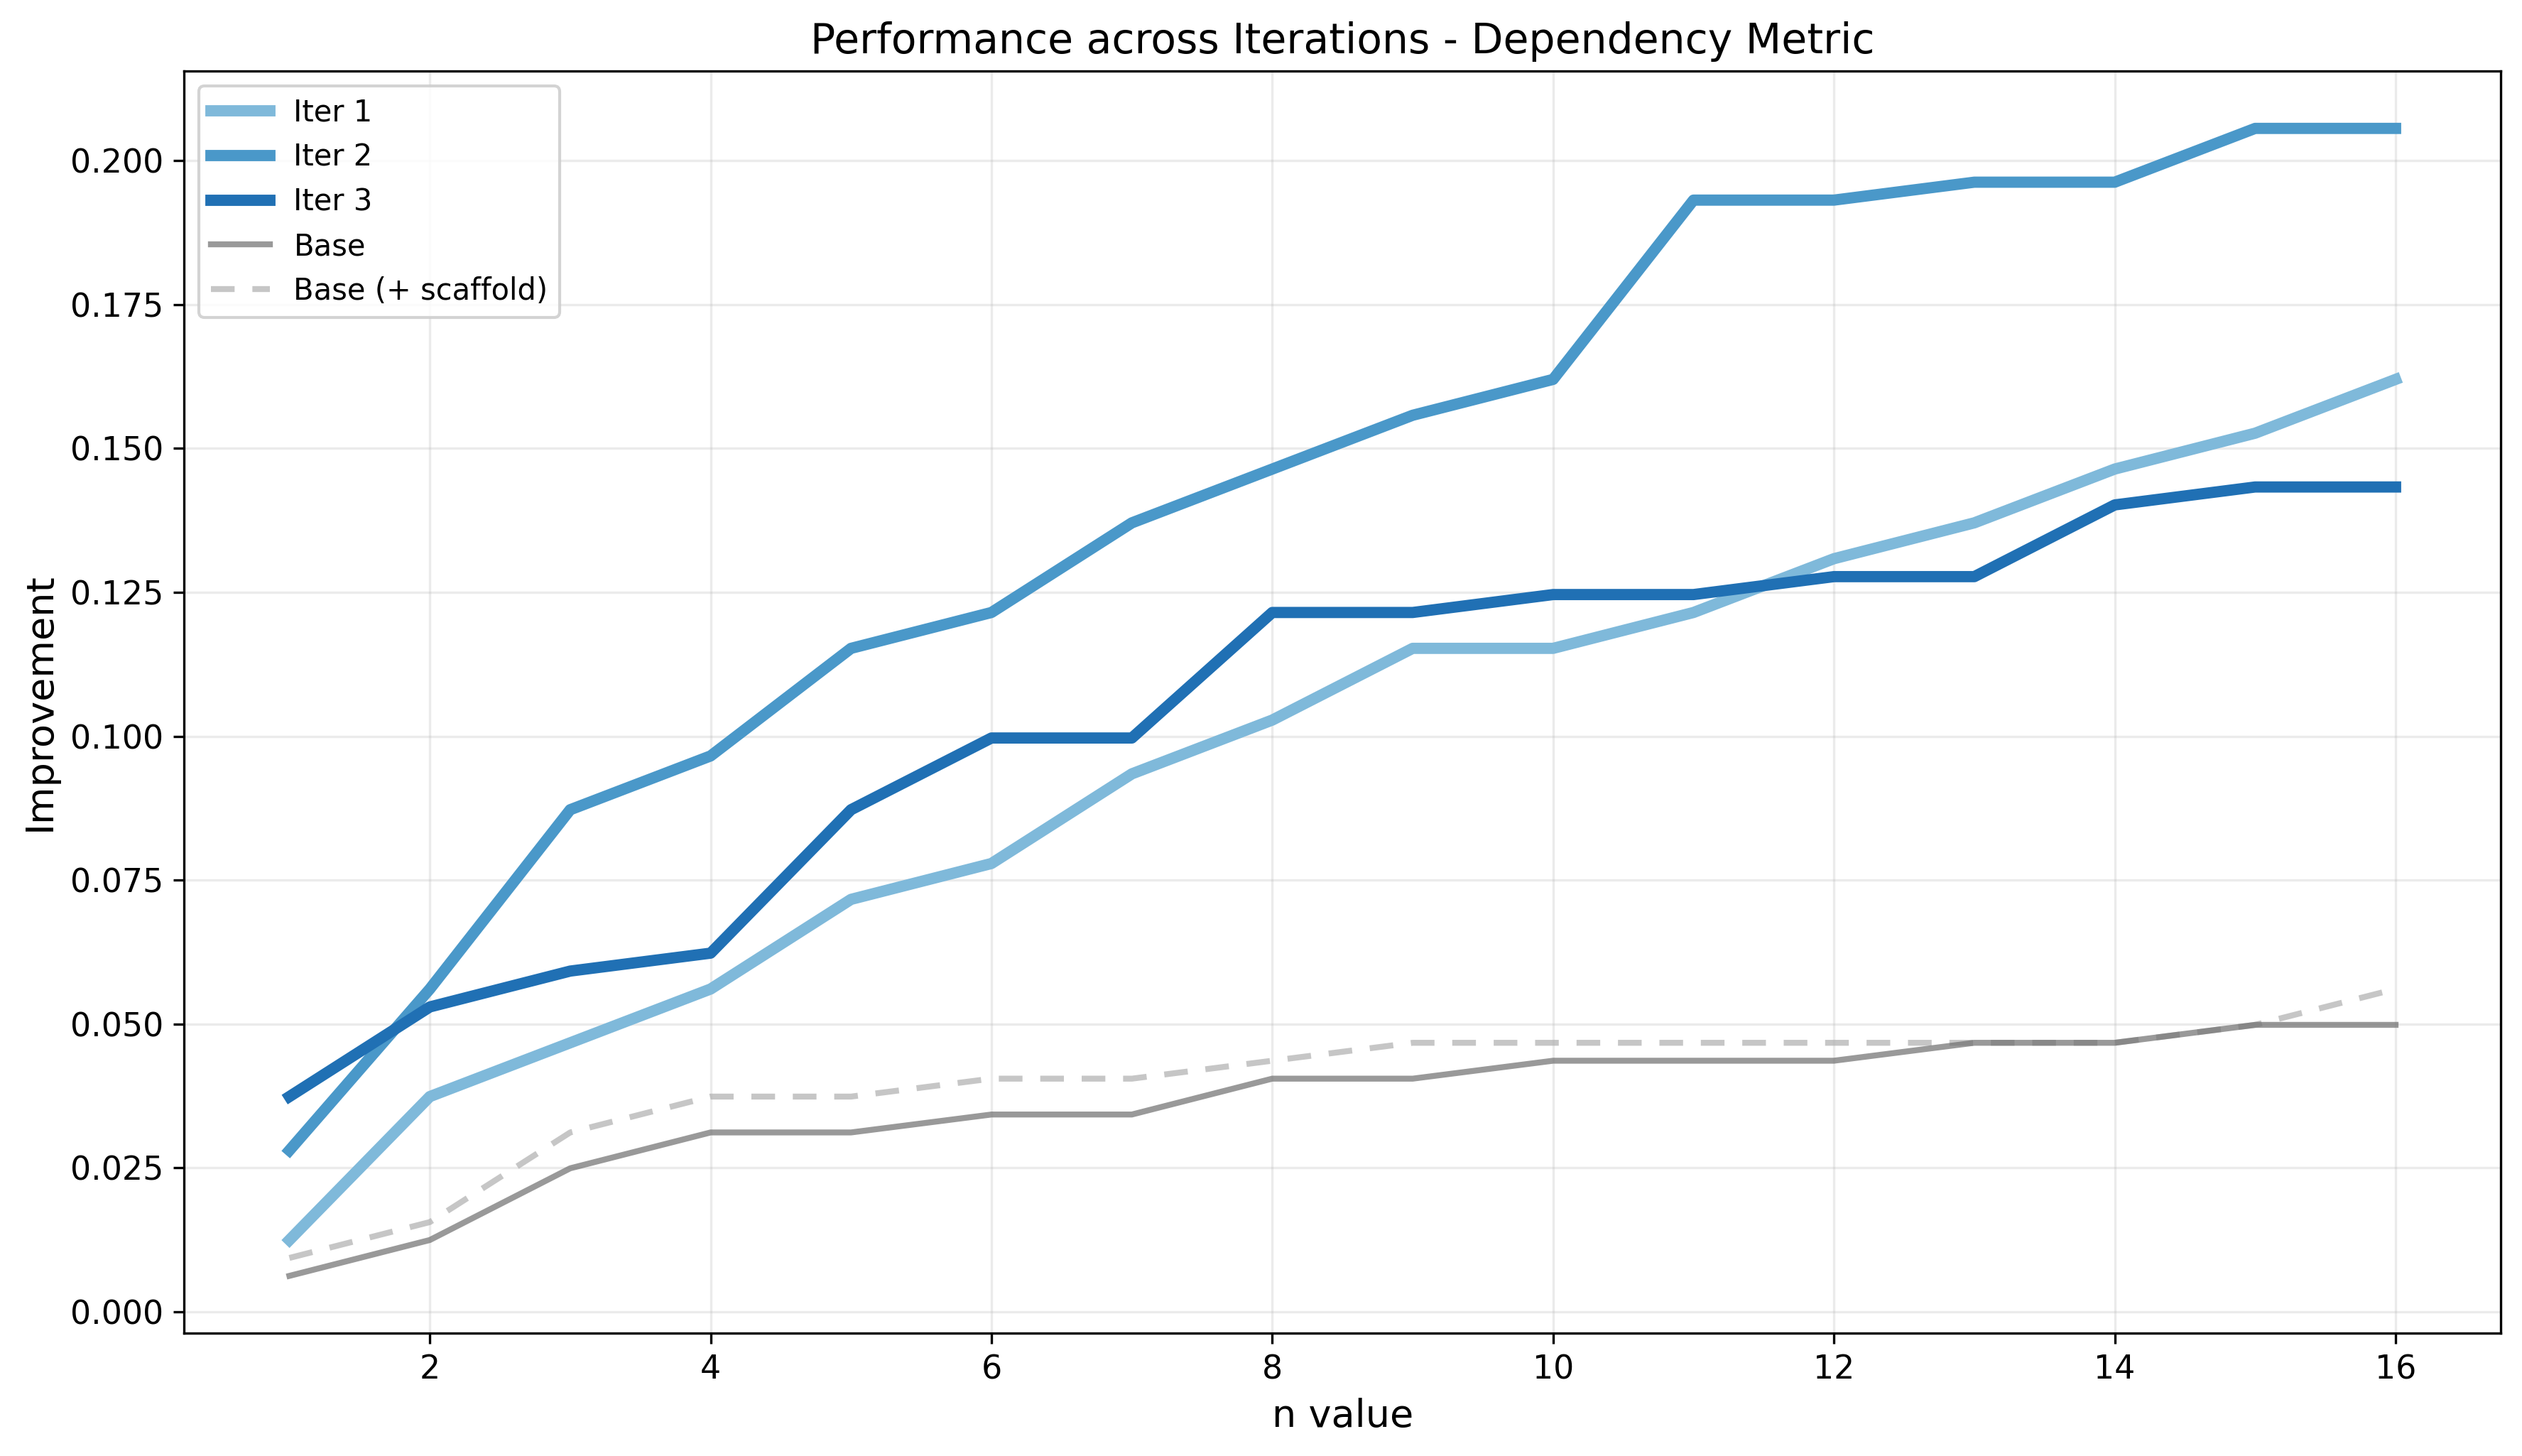
\includegraphics[width=1\linewidth]{figures/Dependency/dependency_iterations.png}
\end{minipage}
\hfill


\begin{minipage}{0.49\linewidth}
    \centering
    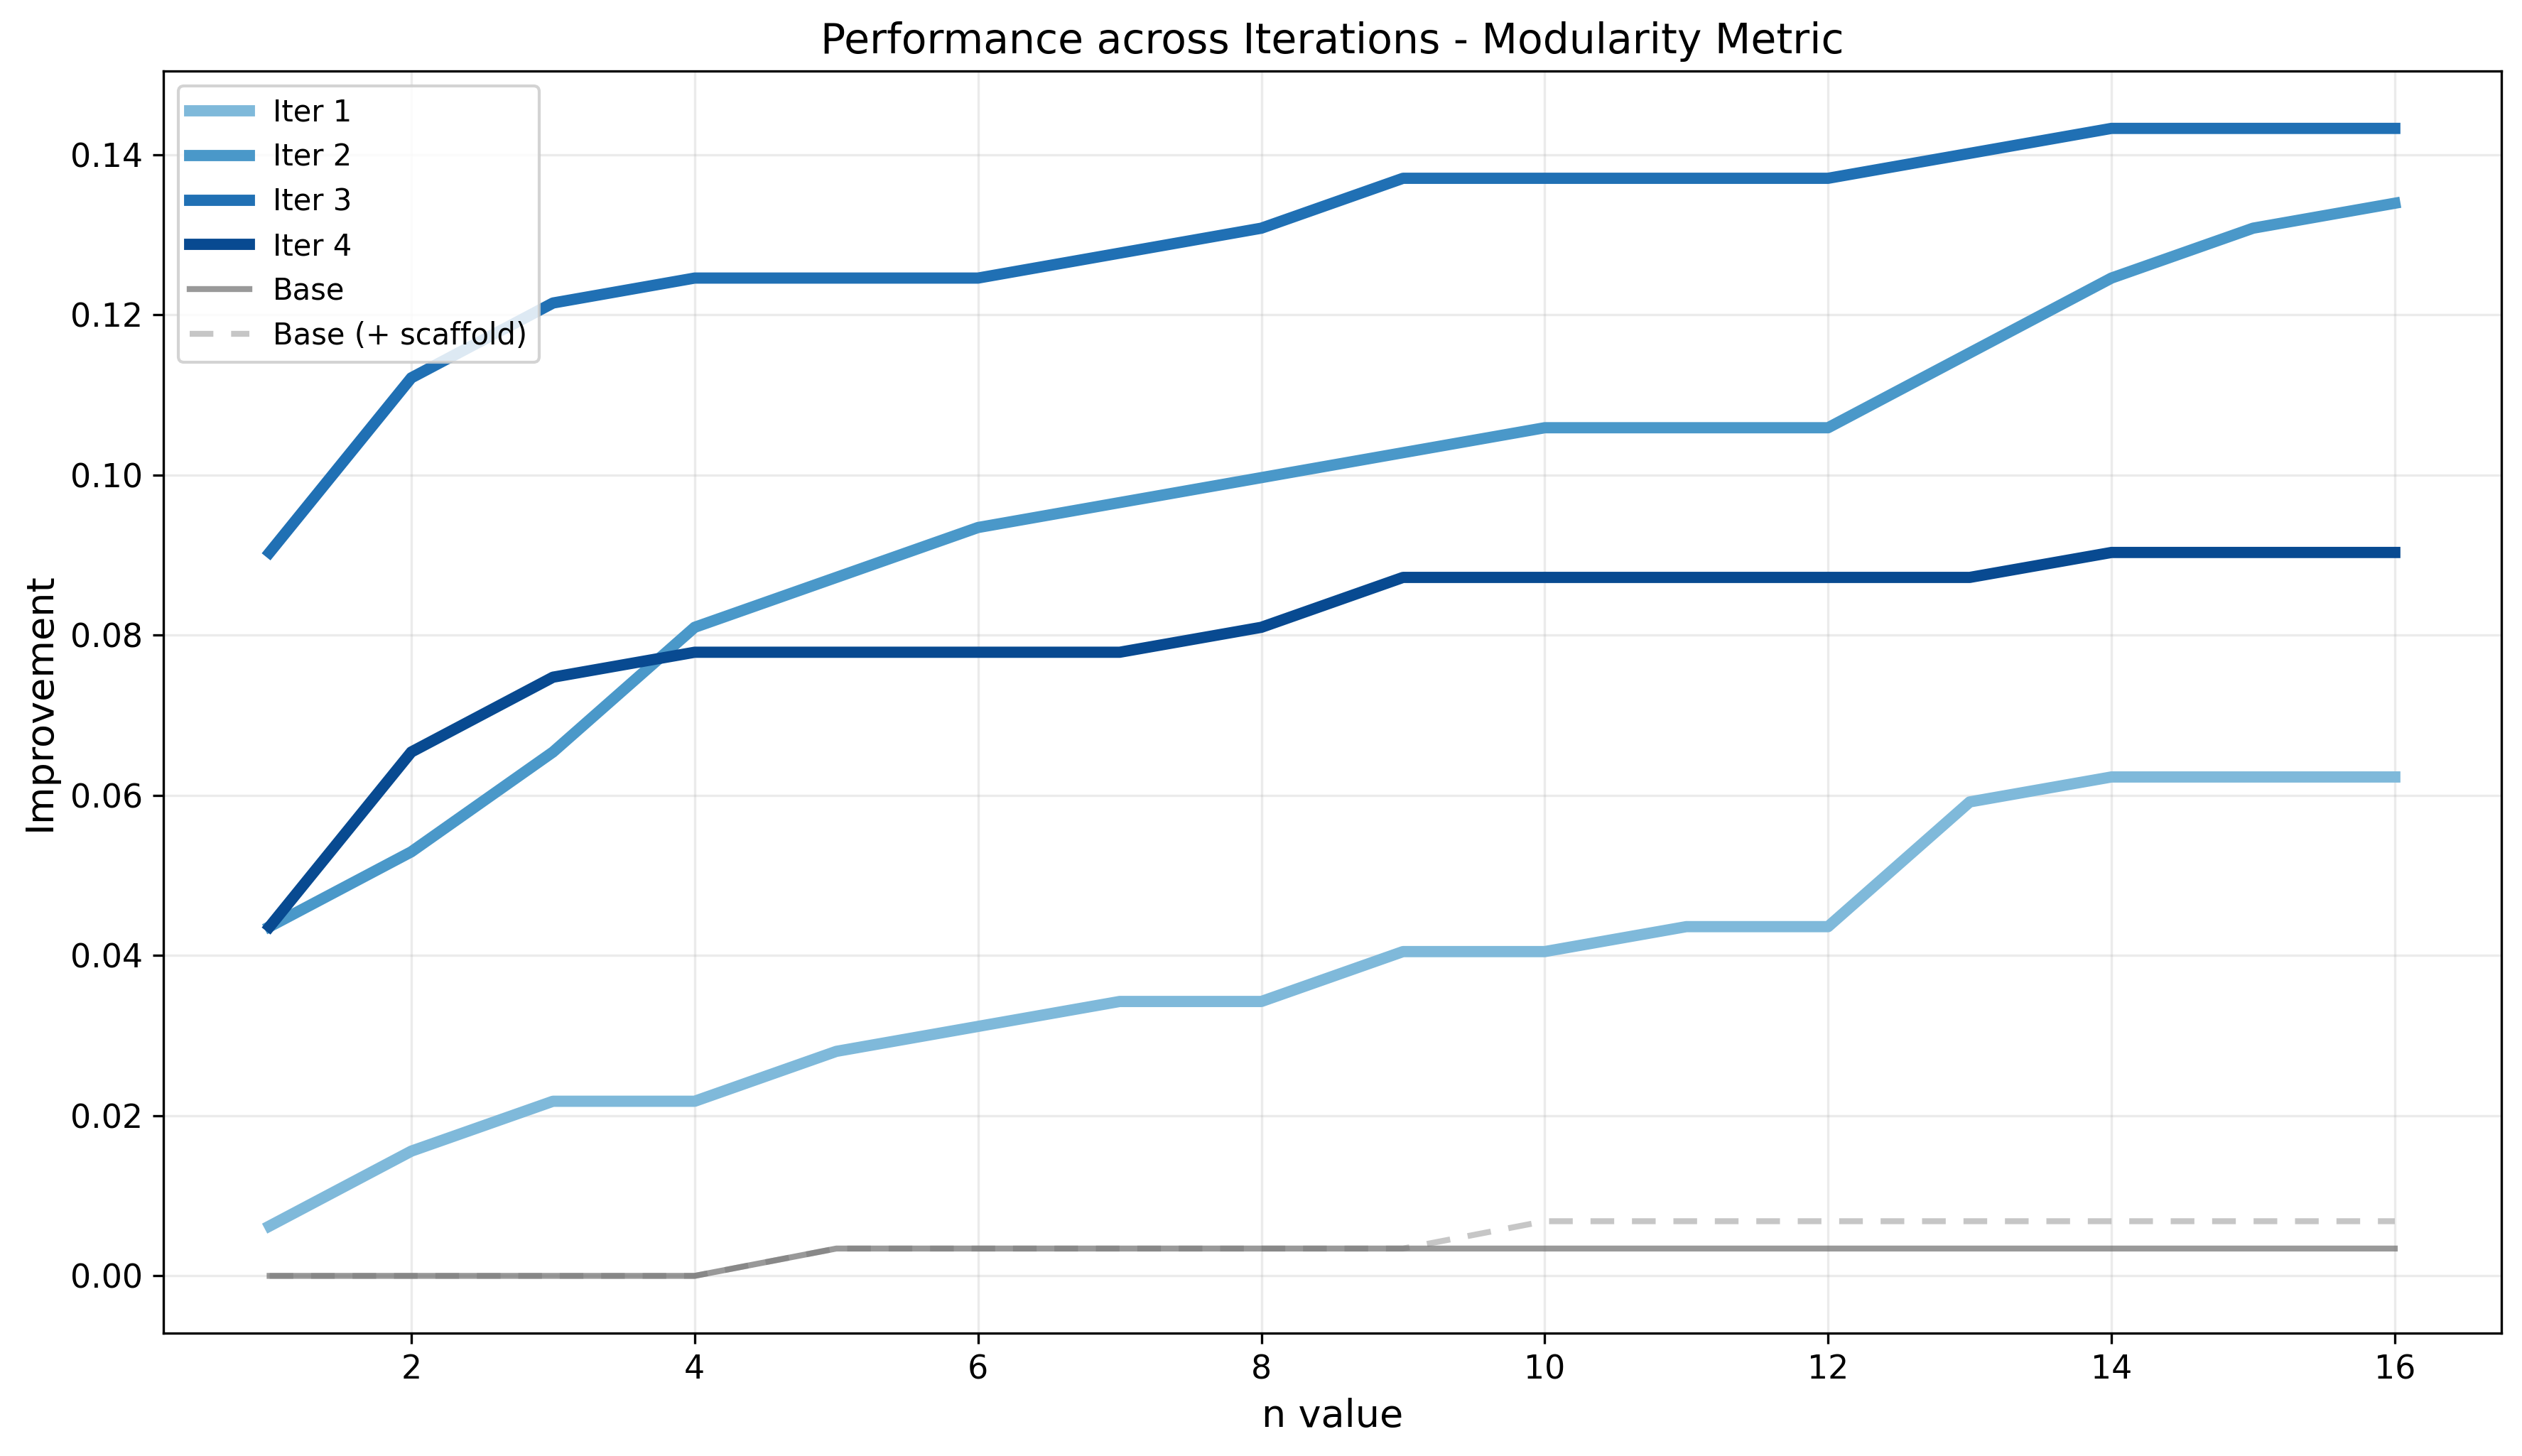
\includegraphics[width=1\linewidth]{figures/Modularity/declarativity2_iterations.png}
\end{minipage}
\hfill
\begin{minipage}{0.49\linewidth}
    \centering
    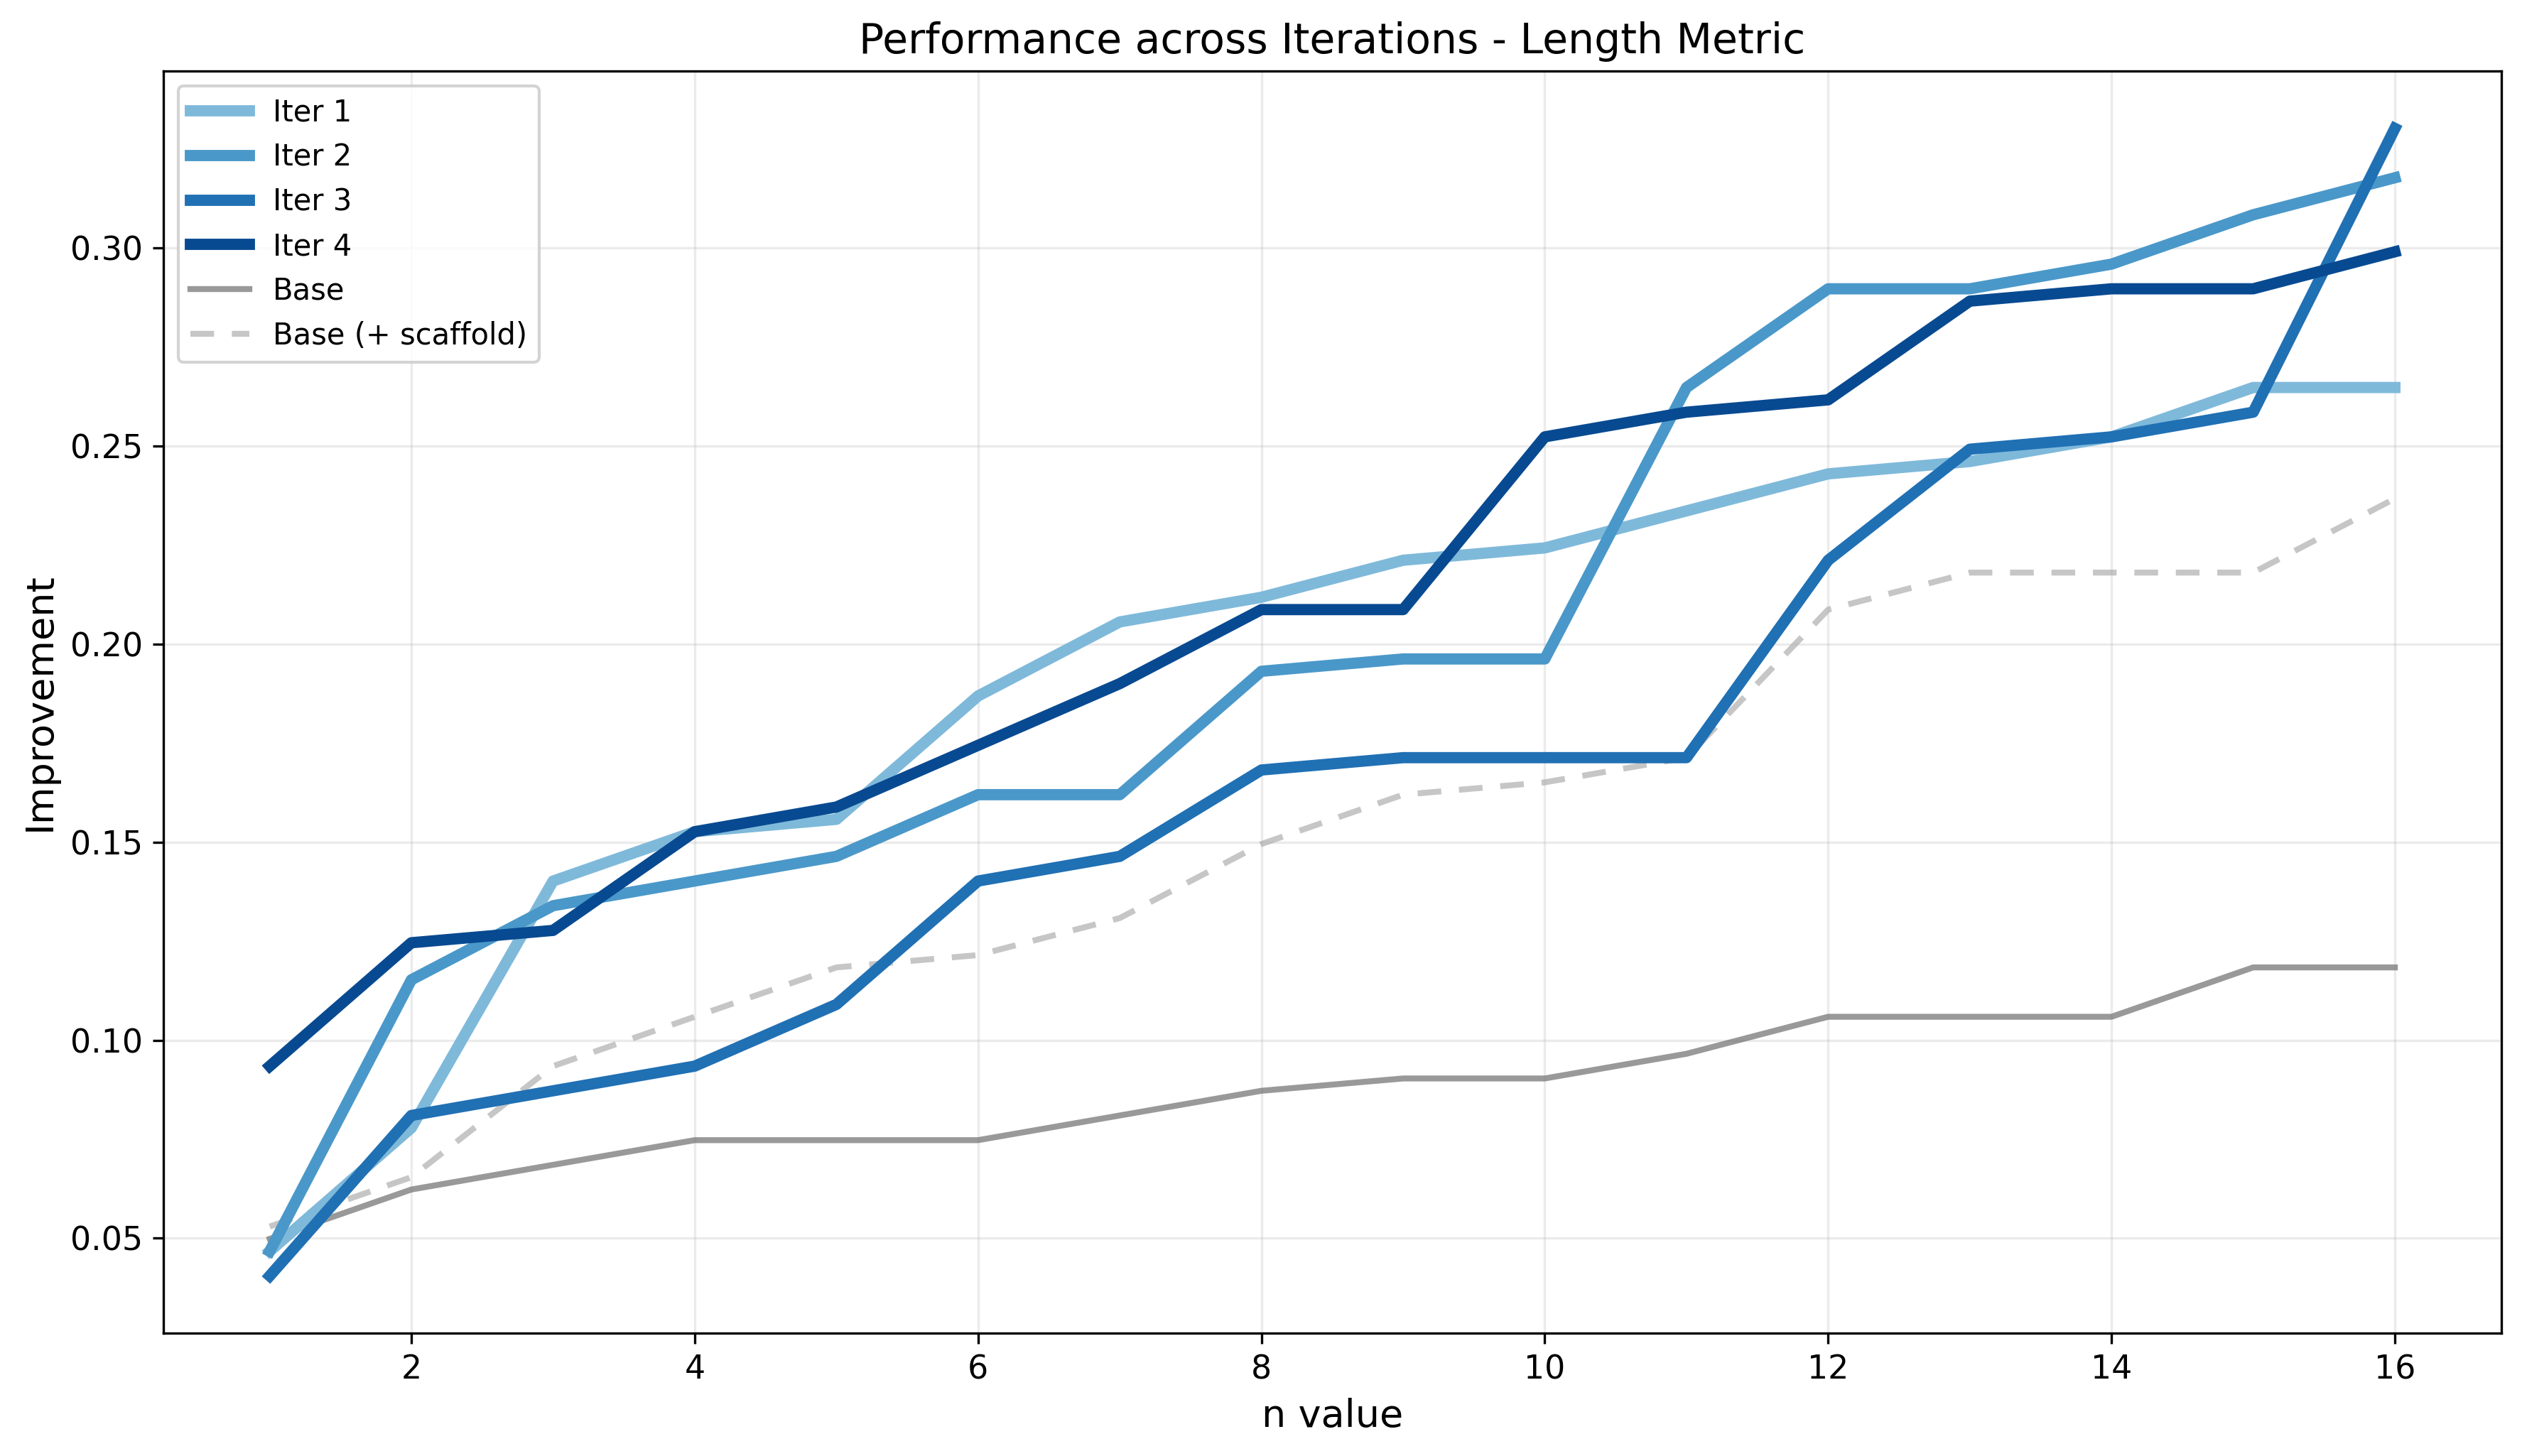
\includegraphics[width=1\linewidth]{figures/Length/length_iterations.png}
\end{minipage}
 \caption{Performance of ImProver 2\ as a function of sample budget across training iterations. Gains are largest in early iterations, with saturation by iterations 2–3 and mild regression thereafter.}
 \label{fig:all_iterations}
\end{figure*}

Table~\ref{tab:iter} and Fig.~\ref{fig:all_iterations} show rapid gains in the first few rounds of self-improvement, followed by saturation.
For all three metrics, performance improves sharply from the base model to the first two or three IRPO iterations.
Length rises from $0.118$ to $0.330$, modularity from $0.003$ to $0.143$, and dependency from $0.050$ to a peak of $0.206$ at iteration 2.
These gains indicate that the model is learning useful refactoring behavior from its own filtered generations, and that the replay-buffered preference data remains informative for multiple rounds.

Improvement is not indefinite, however.
After the peak, later iterations plateau or regress slightly: dependency falls from $0.206$ at iteration 2 to $0.165$ at iteration 3, and both length and modularity decline at iteration 4.
We interpret this as saturation rather than instability.
Once the most common and highest-yield refactoring patterns have been absorbed, later rounds appear to produce fewer genuinely novel improvements and increasingly focus on narrower or noisier examples.

These results also justify selecting checkpoints separately for each metric.
Dependency peaks earlier, while length and modularity benefit from one additional round.
This difference is plausible given the nature of the objectives: dependency minimization often admits relatively direct simplifications, whereas modularity improvements require more global restructuring and therefore appear to be learned more gradually.




\subsection{Per-repository heterogeneity}
\label{sec:repo_hetero}



\begin{table}
\centering
\caption[Average improvement by project and metric.]{\textbf{Average improvement by project and metric.}}
\label{tab:project_improvement}
\small
\begin{tabular}{l|ccc}
\hline
\textbf{Project} & \textbf{Length} & \textbf{Dependency} & \textbf{Modularity} \\
\hline
HepLean    & \textbf{1.283} & 0.379 & 0.030 \\
ConNF      & 0.420 & 0.278 & 0.048 \\
Seymour    & 0.199 & 0.100 & \textbf{0.359} \\
FLT        & 0.131 & 0.133 & 0.066 \\
Foundation & 0.082 & 0.015 & 0.219 \\
Carleson    & 0.048 & 0.188 & 0.095 \\
Mathlib    & 0.016 & \textbf{0.306} & 0.163 \\
\hline
\end{tabular}
\end{table}

Performance varies substantially across repositories (Table~\ref{tab:project_improvement}), suggesting that optimization opportunity may be mediated by project-specific proof style, theorem difficulty distributions, and domain.
For example, Mathlib exhibits very small length gains but relatively strong dependency and modularity improvements, consistent with a library whose proofs are often already concise but still admit structural refactoring.
By contrast, HepLean and ConNF show much larger length and dependency gains, suggesting that these corpora contain more opportunities for proof compression and simplification.
We treat these repository-level results as descriptive rather than definitive, since they likely reflect both stylistic differences and variation in theorem composition across projects.




\subsection{Qualitative optimization behaviors}
\label{sec:qual_behaviors}

[todo: make sure to ref the figure in chapter 3, as well as the corresponding appendix]

Beyond aggregate metrics, ImProver 2\ learns distinct families of refactoring behaviors that align with the intended objective.
For length minimization, the model frequently merges local tactic sequences into shorter automation-heavy proofs, replacing explicit intermediate steps with more compact combinations of simplification and search.
For dependency minimization, it often rewrites proofs to rely on more local reasoning, generic automation, or broader lemmas, reducing the number of explicitly named external facts. This metric may also replace brittle, version-specific \texttt{simp only} or \texttt{rw} chains with broader automation tactics such as \texttt{simp}, a pattern that is consistent with Mathlib's own style guidance~\cite{lean_style_guide} but which means the metric should be interpreted as measuring explicit dependency footprint rather than capturing 
every dimension of proof quality.

For modularity, it introduces intermediate claims and clearer proof boundaries, turning flat tactic scripts into proofs with more reusable substructure. We note that the modularity metric is a structural proxy motivated by 
draft-sketch-prove workflows and lemma decomposition in neural provers; it is not 
a validated proxy for human maintainer preference, and a study of whether 
maintainers prefer modularity-optimized proofs remains an important direction for 
future work.

These behaviors are qualitatively important because they show that the model is not merely exploiting superficial quirks of the metrics.
Instead, the resulting proofs often reflect recognizable mathematical refactoring patterns of the kind a human maintainer might intentionally perform.
The qualitative examples therefore support the interpretation of the quantitative results: ImProver 2\ is learning reusable structural transformations, rather than only memorizing a small set of syntactic shortcuts.





\subsection{Discussion}
\label{sec:discussion}

[todo: discuss the the results, their implications, compare to ImProver and disucss how ImProver 2 naturaally extends ImProver and compensates for its limitations. Discuss the scaffold results too. And the qualitatives touch on them again too, but now in the broader context of the results as a whole, and also failure modes and limtiations of improver 2]


\subsection{Limitations}
\label{sec:limitations}

[todo: limitations (see reviewer comments)]
